  %%%%%%%%%%%%%%%%%%%%%%%%%%%%%%%%%%%%%% -*- coding: utf-8; mode: latex -*- %%
  %
%%%%%    ESTE FICHEIRO ESTÁ FORMATADO PARA LaTeX2e, NÃO PODENDO, POR ISSO,
 %%%                SER PROCESSADO UTILIZANDO LaTeX 2.09.
  %

\documentclass[doublespace,a4paper,11pt,twoside,onecolumn,final,openright]{thesis}
\begin{document}

  %%%%%%%%%%%%%%%%%%%%%%%%%%%%%%%%%%%%%%%%%%%%%%%%%%%%%%%%%%%%%%%%%%%%%%%%%%%%%
  %
%%%%%              M A T E R I A L     I N T R O D U T Ó R I O
 %%%
  %

\frontmatter

\nocite{*}

%------------------------------------------------------------------------------
% Definitions: title, date, author
% Preliminary material: abstract, keywords, aknowledgements, etc.
%
  %%%%%%%%%%%%%%%%%%%%%%%%%%%%%%%%%%%%% -*- coding: utf-8; mode: latex -*- %%
  %
%%%%%                  TÍTULO E DATA OFICIAL DA TESE
 %%%
  %

\def\date{September 2021}
\def\title{Explaining Parkinson’s Disease Computational Diagnostic based on Speech Analysis}

% hypernavigation in PDF docs
\hypersetup{
   debug=false,
   linkcolor=blue,  %%% cor do tableofcontents, \ref, \footnote, etc
   citecolor=red,  %%% cor do \cite
   urlcolor=blue,   %%% cor do \url e \href
   bookmarksopen=true,
   pdftitle={\title},
   pdfauthor={Author's Name},
   pdfsubject={Labore et Dolore},
   pdfkeywords={Labore, Dolore}
}

  %%%%%%%%%%%%%%%%%%%%%%%%%%%%%%%%%%%%%%%%%%%%%%%%%%%%%%%%%%%%%%%%%%%%%%%%%%%%%
  %
%%%%%                          CAPA DA TESE
 %%%
  %

\thispagestyle{empty}

\begin{singlespace}
\vbox to\textheight{%
%--------------------------------------------------
\vskip-1.3in%---------- LOGO E NOME IST/UTL -------
%--------------------------------------------------
\hskip-17mm\vbox to50mm{
\vfil%
\begin{tabular}{l}

\includegraphics[width=9cm]{figs/preliminar/IST_A_CMYK_POS.pdf}
\end{tabular}
\vfil
\vfil
}%
%--------------------------------------------------
\vskip18mm%---------- FIGURAS DA CAPA -------------
%--------------------------------------------------
\vbox to25mm{\LARGE\sl
\vfil
%\centerline{\psfig{file=figs/preliminar/tarantula.eps,height=25mm}}
\vfil
}%
%--------------------------------------------------
\vskip6mm%---------- TÍTULO -----------------------
%--------------------------------------------------
\vbox to25mm{\LARGE\sf
\vfil
\begin{center}
\textbf\title
\end{center}
\vfil
}%
%--------------------------------------------------
\vskip10mm%---------- NOME E GRAU ACTUAL -----------
%--------------------------------------------------
\vbox to25mm{\large
\vfil
\begin{center}
{\Large\sf\textbf {Artur Oliveira Fortunato}}\\   % author's name
\end{center}
\vfil
}%
%--------------------------------------------------
\vskip8mm%---------- GRAU A OBTER -----------------
%--------------------------------------------------
\vbox to8mm{\large\sf
\vfil
\centerline{Thesis to obtain the Master of Science Degree in}
\vskip3mm
\centerline{\LARGE\textbf{Computer Science and Engineering}}
\vfil
}%
%--------------------------------------------------
\vskip15mm%---------- ORIENTADOR -------------------
%--------------------------------------------------
\vbox to8mm{\large\sf
\vfil
\begin{center}
\begin{tabular}{c}
Supervisors: Doctor David Manuel Martins de Matos\\
            Doctor Alberto Abad Gareta\\
\end{tabular}
\end{center}
\vfil
}%
%%--------------------------------------------------
%\vfil
% %--------------------------------------------------
\vskip15mm%---------- J�RI -------------------------
% %--------------------------------------------------
%\vbox{\Large%
%\vfil%
%\begin{center}
%{\Large\sf\textbf{Examination Committee}}\\
%\end{center}
%\vfil%
%}%

\vbox to30mm{\large\sf
\vfil
\begin{center}
{\Large\sf\textbf{Examination Committee}}\\
\quad\\
\begin{tabular}{c}
Chairperson: Doctor name-of-president\\
Supervisor: Doctor David Manuel Martins de Matos\\
Member of the Committee: Doctor name-of-member-of-committee\\
\end{tabular}
\end{center}
\vfil
}%
%--------------------------------------------------
\vskip12mm%---------- DATA -------------------------
%--------------------------------------------------
\begin{center}
{\Large\sf\textbf\date}
\end{center}

%--------------------------------------------------
}%vbox
\end{singlespace}
\newpage

  %%%%%%%%%%%%%%%%%%%%%%%%%%%%%%%%%%%%%%%%%%%%%%%%%%%%%%%%%%%%%%%%%%%%%%%%%%%%%
  %
%%%%%                             AGRADECIMENTOS
 %%%
  %

\chapter*{Agradecimentos}
%\chapter*{Acknowledgements}
\thispagestyle{empty}

% AGRADECER!

Magníficos Agradecimentos

\vfill
\begin{flushright}
  \begin{minipage}{8cm}
    \begin{center}
      Lisboa, \today

      Artur Oliveira Fortunato
    \end{center}
  \end{minipage}
\end{flushright}

\cleardoublepage

  %%%%%%%%%%%%%%%%%%%%%%%%%%%%%%%%%%%%%%%%%%%%%%%%%%%%%%%%%%%%%%%%%%%%%%%%%%%%%
  %
%%%%%                            DEDICATÓRIAS
 %%%
  %

\chapter*{}
\thispagestyle{empty}

% DEDICAR!
\vfill
\mbox{}
\vfill\Large
\begin{flushright}
  \begin{minipage}{8cm}
    \begin{center}

Dedicatória interessante

    \end{center}
  \end{minipage}
\end{flushright}
\normalsize\vfill

\cleardoublepage

  %%%%%%%%%%%%%%%%%%%%%%%%%%%%%%%%%%%%%%%%%%%%%%%%%%%%%%%%%%%%%%%%%%%%%%%%%%%%%
  %
%%%%%                                RESUMO
 %%%
  %

\chapter*{Resumo}
\thispagestyle{empty}

[TRADUZIR PARA PORTUGUÊS] Parkinson’s Disease (PD) is a neurodegenerative disorder that affects the central nervous system. The disease manifests
itself in the patient’s speech, which usually becomes slurred, monotonic, and breathy. This symptoms provide a powerful
biomarker for the detection of PD.
The present work will analyse the subject’s speech, representing it with a set of acoustic features. With this repre-
sentation, a Machine Learning (ML) model will be trained to diagnose PD. By performing cross-language tests on this
classification model, we will evaluate the hypothesis that a ML classifier can correctly diagnose PD. In addition, this
diagnosis will be independent of the language spoken by the subject. Furthermore, we will explore the use of an explain-
ability model, which will “translate” the classification model’s diagnosis to a medical professional. The model will provide
essential information for the clinician to trust and use this tool.
Despite the good results achieved by many ML classification models, their acceptance for the diagnosis of this disease
has not yet been achieved. Clinicians are unable to use the model’s diagnosis, as it lacks a medical-oriented interpretation.
Therefore, this work is motivated by the practical need of a universal, language-independent model that can provide
enough human-understandable information to support clinical usage of ML models on PD diagnosis. This project will
provide a tool that can boost the transfer of such models from test environments to real-life usage.
\newpage

  %%%%%%%%%%%%%%%%%%%%%%%%%%%%%%%%%%%%%%%%%%%%%%%%%%%%%%%%%%%%%%%%%%%%%%%%%%%%%
  %
%%%%%                            ABSTRACT
 %%%
  %

\chapter*{Abstract}
\thispagestyle{empty}

Parkinson’s Disease (PD) is a neurodegenerative disorder that affects the central nervous system. One of the disease's manifestation is in the patient’s speech, which usually becomes slurred, monotonic, and breathy. These symptoms provide a powerful bio-marker for the detection of PD.
The present work analyzes the subject’s speech, representing it through a set of acoustic features. With this representation, a Machine Learning (ML) model will be trained to diagnose PD. By performing cross-language tests on this classification model, we will evaluate the hypothesis that a ML classifier can correctly diagnose PD. In addition, this diagnosis will be independent of the language spoken by the subject. Furthermore, we will explore the use of an explainability model, which will “translate” the classification model’s diagnosis to a medical professional. The model will provide essential information for the clinician to trust and use this tool. Despite the good results achieved by many ML classification models, their acceptance for the diagnosis of this disease has not yet been achieved. Clinicians are unable to use the model’s diagnosis, as it lacks a medical-oriented interpretation. Therefore, this work is motivated by the practical need of a universal, language-independent model that can provide enough human-understandable information to support clinical usage of ML models on PD diagnosis. This project will provide a tool that can boost the transfer of such models from test environments to real-life usage.

Parkinson’s Disease (PD) is a neurodegenerative disorder that affects the central nervous system. One of the disease's manifestation is in the patient’s speech, which usually becomes slurred, monotonic, and breathy. These symptoms provide a powerful bio-marker for the detection of PD. \\
The present work comprised two objectives. %Tirar paragrafo
First, to analyze the performance of a language-independent model for the \gls{pd} diagnostic task. For this work, three datasets were used (one in European Portuguese, one in European Spanish and one in European English). A baseline approach (a model trained and tested with speech from the same language) achieved a maximum accuracy of 90\%. An intermediate step was also taken, where a model was trained with speech from one language and part of the speech contained in a different dataset (in a different language) and tested with the remaining part of the speed from the second dataset. This semi language-independent model's performance was similar to the baseline's performance. This results demonstrated the ability of our model to be re-trained with new data from a new language and be extended to patients
Next, a 

- O trabalho tinha dois objectivos \\
- Primeiro, analisar a performance de um modelo independente de linguagem \\
	- Comparámos duas arquiteturas de um MLP \\
	- Baseline - 90\% accuracy \\
	- Semi-language independent - same performance \\
	- Independent - 2/3 \\

- Segundo, usámos o modelo LIME para explicar o diagnóstico do classificador \\
	- 

- É um step forward para a adaptação de modelos de classificação para novas linguagens e para a integração de modelos de explicação que podem levar à adoção de modelos de classificação computacional em casos de vida real

\newpage

  %%%%%%%%%%%%%%%%%%%%%%%%%%%%%%%%%%%%%%%%%%%%%%%%%%%%%%%%%%%%%%%%%%%%%%%%%%%%%
  %
%%%%%                 FICHA BIBLIOGRAFICA -- PALAVRAS CHAVE
 %%%
  %

\chapter*{Palavras Chave \\ Keywords}
\thispagestyle{empty}

\section*{Palavras Chave}
{\large % EM PORTUGUÊS

\noindent Aprendizagem de máquina

\noindent Discurso

\noindent Explicabilidade

\noindent Interpretabilidade

}

\section*{Keywords}

{\large % EM INGLÊS

\noindent Machine Learning

\noindent Speech

\noindent Explainability

\noindent Interpretability

}

\vfill
%LATEX2HTML}

\cleardoublepage


  %%%%%%%%%%%%%%%%%%%%%%%%%%%%%%%%%%%%%%%%%%%%%%%%%%%%%%%%%%%%%%%%%%%%%%%%%%%%%
  %
%%%%%                           CHANGE OF NUMBERING
 %%%
  %

\pagestyle{plain}
\pagenumbering{roman}

  %%%%%%%%%%%%%%%%%%%%%%%%%%%%%%%%%%%%%%%%%%%%%%%%%%%%%%%%%%%%%%%%%%%%%%%%%%%%%
  %
%%%%%                               INDICES
 %%%
  %

% ``Table of contents'' (Apêndice).

\def\contentsname{Table of Contents}
\tableofcontents
\newpage

% Lista de figuras.
\listoffigures
\newpage

% Lista de tabelas.
\listoftables

% Does it always work? I expect so...
\cleardoublepage

  %
 %%%
%%%%%                            T H E    E N D
  %
  %%%%%%%%%%%%%%%%%%%%%%%%%%%%%%%%%%%%%%%%%%%%%%%%%%%%%%%%%%%%%%%%%%%%%%%%%%%%%

% Local Variables: 
% mode: latex
% TeX-master: "tese"
% End: 


%------------------------------------------------------------------------------
% Global definitions (but do not directly produce text)
% Used in the appendices: nomenclature and index
%
  %%%%%%%%%%%%%%%%%%%%%%%%%%%%%%%%%%%%%%% -*- coding: utf-8; mode: latex -*- %%
  %
%%%%%                        T E R M I N O L O G I A
 %%%
  %

% a ordem não é relevante para o processamento, mas é-o para a gestão do
% conteúdo deste ficheiro.
% ATENÇÃO: maiúsculas e minúsculas são consideradas iguais.

\def\AF{AF\index{AF}}
\def\AFS{AFS\index{AFS}}
\def\AlethGD{AlethGD\index{AlethGD}}
\def\Amorfo{Amorfo\index{Amorfo}}
\def\API{API}
\def\ArgoUML{ArgoUML\index{ArgoUML}}
\def\ATA{ATA\index{ATA}}
\def\AUTHOR{AUTHOR\index{AUTHOR}}

\def\BLARK{BLARK\index{BLARK}}
\def\BRASILex{BRASILex\index{BRASILex}}

\def\DCR{DCR\index{DCR}}
\def\DCS{DCS\index{DCS}}
\def\docuplanner{DocuPlanner\index{arquitectura!DocuPlanner (sistema)}\index{modelos de geração!geração profunda!DocuPlanner (sistema)}\index{sistema!DocuPlanner}\index{document drafting!DocuPlanner (sistema)}\index{sistema!DocuPlanner}}
\def\DTD{DTD\index{DTD}}
\def\DTL{DTL\index{DTL}}
\def\DOM{DOM\index{DOM}}

\def\EAGLES{EAGLES\index{EAGLES}}
\def\EPLEXIC{EPLexIC\index{EPLexIC}}
\def\EuroWordNet{EuroWordNet\index{EuroWordNet}}
\def\EUROTRA{EUROTRA\index{EUROTRA}}
\def\Edite{Edite\index{Edite}}

\def\FrameNet{FrameNet\index{FrameNet}}
\def\FUF{FUF\index{FUF}}

\def\Galaxy{Galaxy\index{Galaxy Communicator}}
\def\Galinha{Galinha\index{Galinha}}
\def\GATE{GATE\index{GATE}}
\def\Genelex{Genelex\index{Genelex}}
\def\GGG{Galinha Galaxy Gateway\index{Galinha!Galaxy Gateway}}
\def\GLOSIX{GLOSIX\index{GLOSIX}}

\def\HTML{HTML\index{HTML}}

\def\IMDI{IMDI\index{IMDI}}
\def\ILEX{ILEX\index{ILEX}}
\def\INTERA{INTERA\index{INTERA}}
\def\INESC{INESC\index{INESC}}
\def\ISLE{ISLE\index{ISLE}}
\def\ISO{ISO\index{ISO}}
\def\ispell{ispell\index{ispell}}

\def\Java{Java\index{Java}}
\def\JDBC{JDBC\index{JDBC}}
\def\JSpell{JSpell\index{JSpell}}

\def\Kerberos{Kerberos\index{Kerberos}}

\def\LDAP{LDAP\index{LDAP}}
\def\LDC{LDC\index{LDC}}
\def\LISP{LISP\index{LISP}}
\def\LUSOlex{LUSOlex\index{LUSOlex}}
\def\langpt{Português\index{língua!Português}}
\def\langes{Espanhol\index{língua!Espanhol}}
\def\langen{Inglês\index{língua!Inglês}}
\def\langfr{Francês\index{língua!Francês}}

\def\m4{GNU \texttt{m4}\index{m4}}
\def\marv{MARv\index{MARv}}
\def\MILE{MILE\index{MILE}}
\def\ModelExplainer{ModelExplainer\index{ModelExplainer}}
\def\monge{Monge\index{monge}}
\def\Multext{Multext\index{Multext}}
\def\Multilex{Multilex\index{Multilex}}
\def\MySQL{MySQL\index{MySQL}}

\def\NEMLAR{NEMLAR\index{NEMLAR}}
\def\nlpfarm{NLPFARM\index{NLPFARM}}
\def\NOMLEX{NOMLEX\index{NOMLEX}}
\def\noweb{\texttt{noweb}\index{noweb}}

\def\ODBC{ODBC\index{ODBC}}
\def\OWL{OWL\index{OWL}}

\def\PAROLE{PA\-RO\-LE\index{PAROLE}}
\def\Palavroso{Palavroso\index{Palavroso}}
\def\pasmo{PAsMo\index{PAsMo}}
\def\PEAR{PEAR\index{PEAR}}
\def\PEBA{PEBA\index{PEBA-II}}
\def\PHP{PHP\index{PHP}}
\def\Poseidon{Poseidon\index{Poseidon}}
\def\plandoc{PLANDoc\index{PLANDoc}}
\def\POWER{POWER\index{POWER}}
\def\Python{Python\index{Python}}

\def\RAGS{RAGS\index{RAGS}}
\def\RDF{RDF\index{RDF}}
\def\RDFS{RDFS\index{RDFS}}

\def\SGML{SGML\index{SGML}}


\def\JavaScript{JavaScript\index{JavaScript}}

\def\SIMPLE{SIM\-PLE\index{SIMPLE}}
\def\SMorph{SMorph\index{SMorph}}
\def\SOAP{SOAP\index{SOAP}}
\def\SPEECHDAT{SPEECHDAT\index{SPEECHDAT}}
\def\SQL{SQL\index{SQL}}
\def\StoryBook{StoryBook\index{StoryBook}}
\def\SURGE{SURGE\index{SURGE}}
\def\susana{SuSAna\index{SuSAna}}

\def\TEI{TEI\index{TEI}}
\def\TIPSTER{TIPSTER\index{TIPSTER}}
\def\TCxxxvii{TC37\index{TC37}}
\def\TCxxxviiSCiv{TC37/SC4\index{TC37!SC4}}
\def\TRIPS{TRIPS\index{TRIPS}\index{modos de interacção!diálogo!TRIPS (sistema)}\index{sistema!TRIPS}}

\def\UML{UML\index{UML}}
\def\Unix{Unix\index{Unix}}

\def\vnACCMS{vnACCMS\index{vnACCMS}}

\def\WeatherReporter{WeatherReporter\index{WeatherReporter}}
\def\WordNet{WordNet\index{WordNet}}
\def\WSDL{WSDL\index{WSDL}}
\def\WSEL{WSEL\index{WSEL}}
\def\WSFL{WSFL\index{WSFL}}

\def\XA{XA\index{XA}}
\def\XMI{XMI\index{XMI}}
\def\XML{XML\index{XML}}
\def\XSD{XSD\index{XSD}}
\def\XSL{XSL\index{XSL}}
\def\XSLT{XSLT\index{XSLT}}

  %
 %%%
%%%%%                                F   I   M
  %
  %%%%%%%%%%%%%%%%%%%%%%%%%%%%%%%%%%%%%%%%%%%%%%%%%%%%%%%%%%%%%%%%%%%%%%%%%%%%%
                 % terms (definitions for use in text)
  %%%%%%%%%%%%%%%%%%%%%%%%%%%%%%%%%%%%%%% -*- coding: utf-8; mode: latex -*- %%
  %
%%%%%                     NOMENCLATURE / GLOSSARY
 %%%
  %

% a ordem não é relevante para o processamento, mas é-o para a gestão do
% conteúdo deste ficheiro.
% ATENÇÃO: maiúsculas e minúsculas são consideradas iguais.

  %%%%%%%%%%%%%%%%%%%%%%%%%%%%%%%%%%%%%%%%%%%%%%%%%%%%%%%%%%%%%%%%%%%%%%%%%%%%%
  %
%%%%%                     A  A  A  A  A  A  A  A  A
 %%%
  %

\nomenclature{AFS}{Andrew File System ou Advanced File
System. O Andrew File System é um sistema de
ficheiros distribuído. Foi inicialmente desenvolvido na Universidade de
Carnegie Mellon. O AFS apresenta várias vantagens sobre outros sistemas de
ficheiros, particularmente no que respeita às áreas de segurança e
escalabilidade.}

\nomenclature{AUTHOR}{\AUTHOR: arquitecura de
  geração de prosa narrativa. Ver a entrada
  correspondente a \StoryBook.}

  %%%%%%%%%%%%%%%%%%%%%%%%%%%%%%%%%%%%%%%%%%%%%%%%%%%%%%%%%%%%%%%%%%%%%%%%%%%%%
  %
%%%%%                     B  B  B  B  B  B  B  B  B
 %%%
  %

\nomenclature{BLARK}{Basic LAnguage Resource Kit.}

  %%%%%%%%%%%%%%%%%%%%%%%%%%%%%%%%%%%%%%%%%%%%%%%%%%%%%%%%%%%%%%%%%%%%%%%%%%%%%
  %
%%%%%                     C  C  C  C  C  C  C  C  C
 %%%
  %

  %%%%%%%%%%%%%%%%%%%%%%%%%%%%%%%%%%%%%%%%%%%%%%%%%%%%%%%%%%%%%%%%%%%%%%%%%%%%%
  %
%%%%%                     D  D  D  D  D  D  D  D  D
 %%%
  %

\nomenclature{DCR}{Data Category
Registry. A \DCR{} é
um componente do Linguistic Annotation
Framework que contém um
conjunto de categorias linguísticas definido
formalmente.}

\nomenclature{DCS}{Data Category Selection:
subconjuntos de uma \DCR{} que reflectem vários domínios temáticos e várias
classes e funções de categorias de dados.}

%--------------------------------------------------
% sec:content-determination
%
\nomenclature{Determinação de conteúdo}{Tarefa que decide que in\-for\-ma\-ção
  deve ser comunicada no documento de saída. Pode ser vista como o aspecto de
  conteúdo do planeador de documentos. No contexto do projecto \RAGS,
  esta designação corresponde a toda a fase de planeamento do
  documento.}

\nomenclature{DocuPlanner}{\docuplanner{} -- Um sistema de preparação de rascunhos de documentos.}

\nomenclature{DOM}{Document Object Model. O Document Object
Model é uma interface neutra relativamente a plataformas ou linguagens
particulares. Esta interface permite acesso dinâmico ao conteúdo, estrutura
e estilo de documentos que sigam este padrão.}

  %%%%%%%%%%%%%%%%%%%%%%%%%%%%%%%%%%%%%%%%%%%%%%%%%%%%%%%%%%%%%%%%%%%%%%%%%%%%%
  %
%%%%%                     E  E  E  E  E  E  E  E  E
 %%%
  %

\nomenclature{Edite}{Sistema desenvolvido para aceder em
  linguagem natural a uma base de dados de recursos turísticos dos quiosques
  multimédia do \INESC. O processo de acesso contempla três etapas: (a)
  análise morfológica responsável pela associação de informação morfo\pdash{}sintáctica às
  palavras da frase; (b) análise sintáctica (algoritmo de Earley), fase em que
  são geradas uma ou mais árvores sintácticas representantes da estrutura da
  frase; (c) análise semântica, onde é criada uma forma lógica que exprime o
  significado da frase em tratamento. O sistema é multilingue, suportando
  interacções em \langpt, \langes, \langen{} e \langfr.}

  %%%%%%%%%%%%%%%%%%%%%%%%%%%%%%%%%%%%%%%%%%%%%%%%%%%%%%%%%%%%%%%%%%%%%%%%%%%%%
  %
%%%%%                     F  F  F  F  F  F  F  F  F
 %%%
  %

\nomenclature{FUF}{Iniciais de \textsl{Funcional Unification
    For\-mal\-ism}.}

\nomenclature{Função de correspondência semântica}{No contexto da arquitectura
  dos dados,
  função que traduz a semântica dos dados que fluem através de uma ligação
  entre dois módulos em comunicação.}

  %%%%%%%%%%%%%%%%%%%%%%%%%%%%%%%%%%%%%%%%%%%%%%%%%%%%%%%%%%%%%%%%%%%%%%%%%%%%%
  %
%%%%%                     G  G  G  G  G  G  G  G  G
 %%%
  %

  %%%%%%%%%%%%%%%%%%%%%%%%%%%%%%%%%%%%%%%%%%%%%%%%%%%%%%%%%%%%%%%%%%%%%%%%%%%%%
  %
%%%%%                     H  H  H  H  H  H  H  H  H
 %%%
  %

  %%%%%%%%%%%%%%%%%%%%%%%%%%%%%%%%%%%%%%%%%%%%%%%%%%%%%%%%%%%%%%%%%%%%%%%%%%%%%
  %
%%%%%                     I  I  I  I  I  I  I  I  I
 %%%
  %

\nomenclature{ispell}{International Ispell é um programa interactivo para
  verificação ortográfica que suporta várias línguas Europeias.
}

  %%%%%%%%%%%%%%%%%%%%%%%%%%%%%%%%%%%%%%%%%%%%%%%%%%%%%%%%%%%%%%%%%%%%%%%%%%%%%
  %
%%%%%                     J  J  J  J  J  J  J  J  J
 %%%
  %

  %%%%%%%%%%%%%%%%%%%%%%%%%%%%%%%%%%%%%%%%%%%%%%%%%%%%%%%%%%%%%%%%%%%%%%%%%%%%%
  %
%%%%%                     K  K  K  K  K  K  K  K  K
 %%%
  %

\nomenclature{Kerberos}{Protocolo de autenticação em
rede. Está desenhado para
providenciar autenticação forte entre aplicações cliente/servidor através de
criptografia de chave secreta.}

  %%%%%%%%%%%%%%%%%%%%%%%%%%%%%%%%%%%%%%%%%%%%%%%%%%%%%%%%%%%%%%%%%%%%%%%%%%%%%
  %
%%%%%                     L  L  L  L  L  L  L  L  L
 %%%
  %

\nomenclature{LDAP}{Lightweight Directory Access
Protocol é um conjunto de protocolos para acesso a
informação organizada em directórios. O \LDAP{} baseia-se na norma
X.500, sendo, no entanto, mais simples e
interoperável com protocolos Internet.}

  %%%%%%%%%%%%%%%%%%%%%%%%%%%%%%%%%%%%%%%%%%%%%%%%%%%%%%%%%%%%%%%%%%%%%%%%%%%%%
  %
%%%%%                     M  M  M  M  M  M  M  M  M
 %%%
  %

\nomenclature{m4}{Processador de macros. \m4{} possui funções internas para inclusão de ficheiros,
  execução de comandos, aritmética, etc.}

  %%%%%%%%%%%%%%%%%%%%%%%%%%%%%%%%%%%%%%%%%%%%%%%%%%%%%%%%%%%%%%%%%%%%%%%%%%%%%
  %
%%%%%                     N  N  N  N  N  N  N  N  N
 %%%
  %

\nomenclature{noweb}{Ferramenta de programação
  literária independente da linguagem de pro\-gra\-ma\-ção.}

  %%%%%%%%%%%%%%%%%%%%%%%%%%%%%%%%%%%%%%%%%%%%%%%%%%%%%%%%%%%%%%%%%%%%%%%%%%%%%
  %
%%%%%                     O  O  O  O  O  O  O  O  O
 %%%
  %

\nomenclature{OWL}{Web Ontology Language. \OWL{} é uma
linguagem que permite a definição de ontologias baseadas na Web para permitir
a integração de dados e a interoperabilidade entre comunidades. \OWL{} parte
de \RDF{} e \RDFS{} e adiciona vocabulário para a descrição de propriedades e
classes: relações entre classes, cardinalidade, igualdade, entre
outros. \OWL{} permite a
definição de ontologias compatíveis com a arquitectura da Web, em geral, e com
a Semantic Web, em particular.}

  %%%%%%%%%%%%%%%%%%%%%%%%%%%%%%%%%%%%%%%%%%%%%%%%%%%%%%%%%%%%%%%%%%%%%%%%%%%%%
  %
%%%%%                     P  P  P  P  P  P  P  P  P
 %%%
  %

\nomenclature{Planeador de frases}{Designação alternativa para o
micro\pdash{}planeador (projecto \RAGS).}

\nomenclature{Planeador de texto}{Designação alternativa para o micro\pdash{}planeador.}

  %%%%%%%%%%%%%%%%%%%%%%%%%%%%%%%%%%%%%%%%%%%%%%%%%%%%%%%%%%%%%%%%%%%%%%%%%%%%%
  %
%%%%%                     R  R  R  R  R  R  R  R  R
 %%%
  %

\nomenclature{RDF}{Resource Definition Framework. \RDF{} é
parte da W3C Metadata Activity (\url{http://www.w3.org/Metadata/}). O
objectivo desta actividade, e do \RDF{} em particular, é a produção de uma
linguagem para o intercâmbio de descrições dos recursos da Web. As descrições
destinam-se a usos
automáticos.}

\nomenclature{RDFS}{\RDF{} Schema. \RDFS{} é uma extensão
semântica do \RDF{}, providenciando mecanismos que permitem a descrição de
grupos de recursos relacionados, bem como as relações entre esses recursos. As
descrições são escritas de acordo com \RDF{}. Os recursos são utilizadas para
determinar as características de outros recursos, tais como domínios e gamas
de propriedades.}

  %%%%%%%%%%%%%%%%%%%%%%%%%%%%%%%%%%%%%%%%%%%%%%%%%%%%%%%%%%%%%%%%%%%%%%%%%%%%%
  %
%%%%%                     S  S  S  S  S  S  S  S  S
 %%%
  %

\nomenclature{StoryBook}{\StoryBook{} é uma implementação da arquitecura de
  geração de prosa narrativa AUTHOR. O sistema
  executa as funções de planeamento da narrativa, assim como as funções de
  geração de língua natural. O texto final é construído utilizando o
  realizador de superfície \FUF/\SURGE. As histórias geradas
  situam-se no domínio do Capuchinho Vermelho~\index{Capuchinho
    Vermelho}\index{Little Red Riding Hood|see{Capuchinho Vermelho}}.}

\nomenclature{SURGE}{Realizador de superfície para Inglês (Systemic
  Unification Realization Grammar of English). Uma apresentação do sistema é
  feita em.}

  %%%%%%%%%%%%%%%%%%%%%%%%%%%%%%%%%%%%%%%%%%%%%%%%%%%%%%%%%%%%%%%%%%%%%%%%%%%%%
  %
%%%%%                     T  T  T  T  T  T  T  T  T
 %%%
  %

  %%%%%%%%%%%%%%%%%%%%%%%%%%%%%%%%%%%%%%%%%%%%%%%%%%%%%%%%%%%%%%%%%%%%%%%%%%%%%
  %
%%%%%                     U  U  U  U  U  U  U  U  U
 %%%
  %

  %%%%%%%%%%%%%%%%%%%%%%%%%%%%%%%%%%%%%%%%%%%%%%%%%%%%%%%%%%%%%%%%%%%%%%%%%%%%%
  %
%%%%%                     U  U  U  U  U  U  U  U  U
 %%%
  %

\nomenclature{vnACCMS}{Sistema que realiza tarefas de segmentação
  de palavras e etiquetação morfológica. O sistema utiliza o formato de
  representação para recursos linguísticos tal como definido no âmbito do
  trabalho da equipa \ISO{} \TCxxxviiSCiv{}. Ver
  \url{http://www.loria.fr/equipes/led/outils.php}.}

  %%%%%%%%%%%%%%%%%%%%%%%%%%%%%%%%%%%%%%%%%%%%%%%%%%%%%%%%%%%%%%%%%%%%%%%%%%%%%
  %
%%%%%                     W  W  W  W  W  W  W  W  W
 %%%
  %

\nomenclature{WordNet}{Léxico semântico para Inglês.}

  %%%%%%%%%%%%%%%%%%%%%%%%%%%%%%%%%%%%%%%%%%%%%%%%%%%%%%%%%%%%%%%%%%%%%%%%%%%%%
  %
%%%%%                     X  X  X  X  X  X  X  X  X
 %%%
  %

\nomenclature{XMI}{\XML{} Metadata Interchange. \XMI{} é um
enquadramento para a definição, intercâmbio, manipulação e integração de
objectos \XML. As normas baseadas em \XMI{} permitem a integração de
ferramentas e repositórios.}

\nomenclature{XML}{Extensible Markup Language é um formato de texto, simples e
flexível, derivado de \SGML{} (\ISO{}~8879).}

\nomenclature{XSD}{\XML{} Schema Definition. Os esquemas \XML{}
expressam vocabulários partilhados e providenciam formas de definir a
estrutura, conteúdo e semântica de documentos \XML. Ver
\url{www.oasis-open.org/cover/schemas.html}.}

\nomenclature{XSLT}{\XSL{} Transformations é uma linguagem para
  transformar documentos \XML. A transformação \XSLT{} descreve as regras para
  transformar uma árvore de entrada numa árvore de saída independente da
  árvore original. A linguagem permite filtrar a árvore original assim como a
  adição de estruturas arbitrárias.}

  %
 %%%
%%%%%                                F   I   M
  %
  %%%%%%%%%%%%%%%%%%%%%%%%%%%%%%%%%%%%%%%%%%%%%%%%%%%%%%%%%%%%%%%%%%%%%%%%%%%%%
              % nomenclature/glossary
  %%%%%%%%%%%%%%%%%%%%%%%%%%%%%%%%%%%%%%% -*- coding: utf-8; mode: latex -*- %%
  %
%%%%%                               I  N  D  E  X
 %%%
  %

% a ordem não é relevante para o processamento, mas é-o para a gestão do
% conteúdo deste ficheiro.
% ATENÇÃO: maiúsculas e minúsculas são consideradas iguais.

% on the whole, only crossref entries should be listed here: the others are
% in the terminology file definitions or directly in the text itself

  %%%%%%%%%%%%%%%%%%%%%%%%%%%%%%%%%%%%%%%%%%%%%%%%%%%%%%%%%%%%%%%%%%%%%%%%%%%%%
  %
%%%%%                     A  A  A  A  A  A  A  A  A
 %%%
  %

\index{analisador morfológico!Amorfo|see{Amorfo}}

  %%%%%%%%%%%%%%%%%%%%%%%%%%%%%%%%%%%%%%%%%%%%%%%%%%%%%%%%%%%%%%%%%%%%%%%%%%%%%
  %
%%%%%                     B  B  B  B  B  B  B  B  B
 %%%
  %

  %%%%%%%%%%%%%%%%%%%%%%%%%%%%%%%%%%%%%%%%%%%%%%%%%%%%%%%%%%%%%%%%%%%%%%%%%%%%%
  %
%%%%%                     C  C  C  C  C  C  C  C  C
 %%%
  %

  %%%%%%%%%%%%%%%%%%%%%%%%%%%%%%%%%%%%%%%%%%%%%%%%%%%%%%%%%%%%%%%%%%%%%%%%%%%%%
  %
%%%%%                     D  D  D  D  D  D  D  D  D
 %%%
  %

\index{Data Category Registry|see{DCR}}
\index{Data Category Selection|see{DCS}}

  %%%%%%%%%%%%%%%%%%%%%%%%%%%%%%%%%%%%%%%%%%%%%%%%%%%%%%%%%%%%%%%%%%%%%%%%%%%%%
  %
%%%%%                     E  E  E  E  E  E  E  E  E
 %%%
  %

\index{recomendações EAGLES|see{EAGLES}}
\index{entidade morfológica|see{unidade morfológica}}
\index{entidade sintáctica|see{unidade sintáctica}}
\index{entidade semântica|see{unidade semântica}}

  %%%%%%%%%%%%%%%%%%%%%%%%%%%%%%%%%%%%%%%%%%%%%%%%%%%%%%%%%%%%%%%%%%%%%%%%%%%%%
  %
%%%%%                     F  F  F  F  F  F  F  F  F
 %%%
  %

  %%%%%%%%%%%%%%%%%%%%%%%%%%%%%%%%%%%%%%%%%%%%%%%%%%%%%%%%%%%%%%%%%%%%%%%%%%%%%
  %
%%%%%                     G  G  G  G  G  G  G  G  G
 %%%
  %

\index{Multext!GLOSIX|see{GLOSIX}}
\index{General Lingware Open System Environment|see{GLOSIX}}

  %%%%%%%%%%%%%%%%%%%%%%%%%%%%%%%%%%%%%%%%%%%%%%%%%%%%%%%%%%%%%%%%%%%%%%%%%%%%%
  %
%%%%%                     H  H  H  H  H  H  H  H  H
 %%%
  %

\index{arquitectura!HYLITE+ (sistema)}
\index{sistema!HYLITE+}
\index{tempo real|see{sistemas de tempo real}}
\index{sistemas de tempo real!HYLITE+}

  %%%%%%%%%%%%%%%%%%%%%%%%%%%%%%%%%%%%%%%%%%%%%%%%%%%%%%%%%%%%%%%%%%%%%%%%%%%%%
  %
%%%%%                     I  I  I  I  I  I  I  I  I
 %%%
  %

%\index{projecto!INTERA|see{INTERA}}
%\index{projecto!ISLE|see{ISLE}}
\index{ISO!TC37|see{TC37}}
\index{analisador morfológico!ispell|see{ispell}}
\index{international ispell|see{ispell}}

  %%%%%%%%%%%%%%%%%%%%%%%%%%%%%%%%%%%%%%%%%%%%%%%%%%%%%%%%%%%%%%%%%%%%%%%%%%%%%
  %
%%%%%                     J  J  J  J  J  J  J  J  J
 %%%
  %

\index{Java Database Connectivity|see{JDBC}}
\index{analisador morfológico!JSpell|see{JSpell}}

  %%%%%%%%%%%%%%%%%%%%%%%%%%%%%%%%%%%%%%%%%%%%%%%%%%%%%%%%%%%%%%%%%%%%%%%%%%%%%
  %
%%%%%                     K  K  K  K  K  K  K  K  K
 %%%
  %

  %%%%%%%%%%%%%%%%%%%%%%%%%%%%%%%%%%%%%%%%%%%%%%%%%%%%%%%%%%%%%%%%%%%%%%%%%%%%%
  %
%%%%%                     L  L  L  L  L  L  L  L  L
 %%%
  %

\index{Lightweight Directory Access Protocol|see{LDAP}}
\index{Linguistic Data Consortium|see{LDC}}

  %%%%%%%%%%%%%%%%%%%%%%%%%%%%%%%%%%%%%%%%%%%%%%%%%%%%%%%%%%%%%%%%%%%%%%%%%%%%%
  %
%%%%%                     M  M  M  M  M  M  M  M  M
 %%%
  %

\index{GNU m4|see{m4}}
\index{Multilingual ISLE Lexical Entry|see{MILE}}
\index{gerador morfológico|see{monge}}
\index{realização de superfície!morfológica|see{monge}}
\index{projecto!Multext|see{Multext}}

  %%%%%%%%%%%%%%%%%%%%%%%%%%%%%%%%%%%%%%%%%%%%%%%%%%%%%%%%%%%%%%%%%%%%%%%%%%%%%
  %
%%%%%                     N  N  N  N  N  N  N  N  N
 %%%
  %

\index{programação literária!noweb|see{noweb}}

  %%%%%%%%%%%%%%%%%%%%%%%%%%%%%%%%%%%%%%%%%%%%%%%%%%%%%%%%%%%%%%%%%%%%%%%%%%%%%
  %
%%%%%                     O  O  O  O  O  O  O  O  O
 %%%
  %

\index{Open Database Connectivity|see{ODBC}}

  %%%%%%%%%%%%%%%%%%%%%%%%%%%%%%%%%%%%%%%%%%%%%%%%%%%%%%%%%%%%%%%%%%%%%%%%%%%%%
  %
%%%%%                     P  P  P  P  P  P  P  P  P
 %%%
  %

\index{paradigma de flexão!fonético|see{forma fonética}}
\index{paradigma de flexão!gráfico|see{forma gráfica}}
\index{projecto!PAROLE|see{PAROLE}}
\index{LE-PAROLE|see{PAROLE}}
\index{sistema!PEBA-II|see{PEBA-II}}
\index{modos de interacção!monólogo!PEBA-II (sistema)|see{PEBA-II}}
\index{modelos de geração!geração profunda!PEBA-II (sistema)|see{PEBA-II}}
\index{perfil do utilizador|see{modelo do utilizador}}
\index{preferências do utilizador|see{modelo do utilizador}}
\index{sistema!PLANDoc|see{PLANDoc}}
\index{modelos de geração!geração profunda!PLANDoc (sistema)|see{PLANDoc}}
\index{planeador de texto|see{micro\pdash{}planeador}}
\index{sistema!POWER|see{POWER}}
\index{modos de interacção!monólogo!POWER (sistema)|see{POWER}}
\index{modelos de geração!geração profunda!POWER (sistema)|see{POWER}}

  %%%%%%%%%%%%%%%%%%%%%%%%%%%%%%%%%%%%%%%%%%%%%%%%%%%%%%%%%%%%%%%%%%%%%%%%%%%%%
  %
%%%%%                     R  R  R  R  R  R  R  R  R
 %%%
  %

\index{RDF Schema|see{RDFS}}

  %%%%%%%%%%%%%%%%%%%%%%%%%%%%%%%%%%%%%%%%%%%%%%%%%%%%%%%%%%%%%%%%%%%%%%%%%%%%%
  %
%%%%%                     S  S  S  S  S  S  S  S  S
 %%%
  %

\index{ISO!8879|see{SGML}}
\index{projecto!SIMPLE|see{SIMPLE}}
\index{analisador morfológico!SMorph|see{SMorph}}
\index{arquitectura modular!realizador de superfície!SURGE (sistema)|see{SURGE}}
\index{sistema!SURGE|see{SURGE}}

  %%%%%%%%%%%%%%%%%%%%%%%%%%%%%%%%%%%%%%%%%%%%%%%%%%%%%%%%%%%%%%%%%%%%%%%%%%%%%
  %
%%%%%                     T  T  T  T  T  T  T  T  T
 %%%
  %

\index{Text Encoding Initiative|see{TEI}}

  %%%%%%%%%%%%%%%%%%%%%%%%%%%%%%%%%%%%%%%%%%%%%%%%%%%%%%%%%%%%%%%%%%%%%%%%%%%%%
  %
%%%%%                     U  U  U  U  U  U  U  U  U
 %%%
  %

  %%%%%%%%%%%%%%%%%%%%%%%%%%%%%%%%%%%%%%%%%%%%%%%%%%%%%%%%%%%%%%%%%%%%%%%%%%%%%
  %
%%%%%                     U  U  U  U  U  U  U  U  U
 %%%
  %

  %%%%%%%%%%%%%%%%%%%%%%%%%%%%%%%%%%%%%%%%%%%%%%%%%%%%%%%%%%%%%%%%%%%%%%%%%%%%%
  %
%%%%%                     W  W  W  W  W  W  W  W  W
 %%%
  %

  %%%%%%%%%%%%%%%%%%%%%%%%%%%%%%%%%%%%%%%%%%%%%%%%%%%%%%%%%%%%%%%%%%%%%%%%%%%%%
  %
%%%%%                     X  X  X  X  X  X  X  X  X
 %%%
  %

\index{analisador morfológico!XA|see{XA}}
  %
 %%%
%%%%%                                F   I   M
  %
  %%%%%%%%%%%%%%%%%%%%%%%%%%%%%%%%%%%%%%%%%%%%%%%%%%%%%%%%%%%%%%%%%%%%%%%%%%%%%
                 % xref index terms

%------------------------------------------------------------------------------
% Prepare for normal page numbering.
%
\pagenumbering{arabic}
\pagestyle{headings}
\mainmatter

  %%%%%%%%%%%%%%%%%%%%%%%%%%%%%%%%%%%%%%%%%%%%%%%%%%%%%%%%%%%%%%%%%%%%%%%%%%%%%
  %
%%%%%                  P A R T   I  --  Lorem Ipsum
 %%%
  %

%
\part{Lorem Ipsum}
\thispagestyle{empty}
%\vbox to\textheight{
%\vfil
\chapter*{Minim Veniam}
\thispagestyle{empty}

Lorem ipsum dolor sit amet, consectetur adipisicing elit, sed do eiusmod tempor incididunt ut labore et dolore magna aliqua. Ut enim ad minim veniam, quis nostrud exercitation ullamco laboris nisi ut aliquip ex ea commodo consequat. Duis aute irure dolor in reprehenderit in voluptate velit esse cillum dolore eu fugiat nulla pariatur. Excepteur sint occaecat cupidatat non proident, sunt in culpa qui officia deserunt mollit anim id est laborum.

%}
\newpage
\thispagestyle{empty}



%------------------------------------------------------------------------------
% Chapters are here
%
  %%%%%%%%%%%%%%%%%%%%%%%%%%%%%%%%%%%%%%% -*- coding: utf-8; mode: latex -*- %%
  %
%%%%%                         CHAPTER
 %%%
  %

\chapter{Introduction}
%\addcontentsline{lof}{chapter}{\thechapter\quad Lorem Ipsum}
%\addcontentsline{lot}{chapter}{\thechapter\quad Lorem Ipsum}
\label{ch:lorem}

%\begin{quotation}
%  {\small\it Neque porro quisquam est qui dolorem ipsum quia dolor sit amet, consectetur, adipisci velit...}

%{\small\it -- Cerico}
%\end{quotation}


Neurodegenerative diseases are the most debilitating disorders that ail human kind, and the fourth leading cause of death. Neurodegenerative diseases affect the patient's thinking, movement, cognitive behavior, and memory, causing impairments and disabilities. These diseases include serious disorders like \gls{ad} and \gls{pd} \cite{parkinson_incidence}.

\gls{pd} is the second most common neurodegenerative disease. It was estimated that 1\% of people over 60 years old are affected with \gls{pd} \cite{epidemiology_pd}. In 2015, more than 6 million people suffered from this disease worldwide. This value is projected to double by 2040, mainly driven by the increase of life expectancy \cite{parkinson_worldwide}. One of the consequences of \gls{pd} is the development of dementia. Almost half the \gls{pd} patients develop dementia in the first 10 years after diagnosis \cite{parkinson_10_years}, reaching over 80\% after 20 years \cite{parkinson_20_years}.

Early detection of \gls{pd} can be critical for the life quality of the patient. Hence, the earlier the diagnostic is made, the earlier the treatment can begin, thus starting to control the evolution of the disease and improving the comfort of the patient. Furthermore, the majority of the treatment costs occur during the later stages of the disease, reinforcing the importance of early diagnosis \cite{parkinson_early}.

Over the last years, medicine and health care have been a prime focus for \gls{ai} and \gls{ml}. Numerous models have been tested to these areas, demonstrating impressive results in early detection of many diseases, among other tasks. However, the majority of these experiments focuses only on maximizing accuracy performance. Hence, a large problem remains unsolved on the real application of the previously referred models, as explainability has yet to become a focus for any of these works \cite{LIME_explainability}.
Replacing medical decision‐making with non-explainable, black-box \gls{ml} models, can be contravening with the profound ethical responsibilities of clinicians \cite{black_box_model_problem}. Consequently, the lack of explainability and interpretability of \gls{ml} models used in these areas can seriously limit their chances of adoption in real practice \cite{interpretability_importance}. Therefore, the application of explainable models will increase the possibility for medical professionals to understand a model's output, thus increasing the acceptance of \gls{ai} systems in such tasks \cite{explainable_ai_systems}.

This work aimed to improve our ability to automatically and more accurately diagnose \gls{pd}, by building a classifier that differentiates \gls{pd} patients from healthy people. Additionally, by using an explainability model, human-understandable explanations for the given classification (Parkinson or Healthy) of each patient were generated to foster the use of \gls{ml} models to support \gls{pd}'s diagnosis.

The document is structured as follows. Section 2 describes \gls{pd} and state-of-the-art methodologies for \gls{pd} computational diagnosis. Next, section 3 dives into the concept of \gls{xai}, and reviews multiple approaches developed in this area. Section 4 describes the experimental setup of this work, followed by section 5, which reports the results and their discussion. Finally, Section 6 presents the conclusions and future work.

  %
 %%%
%%%%%                        THE END
  %
  %%%%%%%%%%%%%%%%%%%%%%%%%%%%%%%%%%%%%%%%%%%%%%%%%%%%%%%%%%%%%%%%%%%%%%%%%%%%%

%%% Local Variables: 
%%% mode: latex
%%% TeX-master: "tese"
%%% End: 
                    % first chapter of the first part
  %%%%%%%%%%%%%%%%%%%%%%%%%%%%%%%%%%%%%%% -*- coding: utf-8; mode: latex -*- %%
  %
%%%%%                        CHAPTER
 %%%
  %

\chapter{Parkinson's Disease}
%\addcontentsline{lof}{chapter}{\thechapter\quad Facere Possimus}
%\addcontentsline{lot}{chapter}{\thechapter\quad Facere Possimus}
\label{ch:facere}

%\begin{quotation}
%  {\small\it Neque porro quisquam est qui dolorem ipsum quia dolor sit amet, consectetur, adipisci velit...}

%{\small\it -- Cerico}
%\end{quotation}



\gls{pd} is a common cause of dementia. It consists of a neurodegenerative disorder that affects the central nervous system. Symptoms begin gradually and worsen over time \cite{parkinson}.

Dementia is a syndrome that reduces the cognitive function. It affects a wide range of mental capacities, such as memory, comprehension, calculation, and language. Several factors can contribute to the development of dementia: factors that cannot be changed, such as age (the percentage of people over 60 years old suffering from dementia is estimated to be 5-8\% \cite{dementia_who}) and genetics (having a family history of dementia increases one's probability of developing some form of dementia), and factors that can be changed, such as a poor diet and lack of exercise, smoking, diabetes, vitamin and nutritional deficiencies, excessive alcohol consumption and cardiovascular risk factors \cite{dementia_mayo}. 

Dementia impacts the patient physically and psychologically, but also its carers and family (as it creates a high level of dependency for the patient), and society at economic and social levels \cite{dementia_who}.

  %%%%%%%%%%%%%%%%%%%%%%%%%%%%%%%%%%%%%%%%%%%%%%%%%%%%%%%%%%%%%%%%%%%%%%%%%%%%%
  %
%%%%%                        FIRST SECTION
 %%%
  %

\section{Symptoms}

As previously stated, symptoms begin gradually and worsen over time \cite{parkinson}. The most common symptoms include resting tremors (where hands or arms start shaking when resting), bradykinesia (or slowness of movement), muscle stiffness, which results in difficulty in moving and producing facial expressions, postural instability, which reduces the ability to maintain a steady posture, and dystonia, a condition in which patients have involuntary and repetitive muscle movements. In particular, \gls{pd} also affects speech ability. Slurring and mumbling are observed in \gls{pd} patients' speech, which is often observed to be monotone and breathy. The speech rate is also affected, as most patients speak slowly, although others speak too fast. Finally, cognitive problems have been associated with the disease, manifested as a difficulty in finding the correct words (which also contributes to slowing the speech) \cite{parkinson_symptoms}.

  %%%%%%%%%%%%%%%%%%%%%%%%%%%%%%%%%%%%%%%%%%%%%%%%%%%%%%%%%%%%%%%%%%%%%%%%%%%%%
  %
%%%%%                      SECOND SECTION
 %%%
  %

\section{Speech Impairments}

\gls{pd} patients exhibits multiple speech impairments, both at acoustic and at language levels. Acoustic parameters of speech, such as the \gls{f0} \cite{parkinson_disfluency_harel}, pause duration \cite{parkinson_disfluency_harel} or vowel space time \cite{parkinson_acoustic_analysis_goberman} have been shown to distinguish \gls{pd} from \gls{hc}. 90\% of \gls{pd} patients are reported to have speech and voice disorders \cite{parkinson_90_percent}, which show that this biomarker can be an important source of information to detect \gls{pd}. 
Instances of incomplete closure of vocal folds along with bowing folds during phonation have been reported \cite{features_explained}, leading to noise presence, typically characterized by measures such as \gls{gnr}, \gls{nhr}, \gls{hnr} and \gls{vti}. An increase in the average values of \gls{f0}, jitter, and shimmer have also been measured in PD patients.

  %%%%%%%%%%%%%%%%%%%%%%%%%%%%%%%%%%%%%%%%%%%%%%%%%%%%%%%%%%%%%%%%%%%%%%%%%%%%%
  %
%%%%%                         ANOTHER SECTION
 %%%
  %
\section{Diagnosis}

To measure the progression of \gls{pd}, \gls{hny} was proposed \cite{hoehn_yahr}. This scale describes the disease through five stages, ranging from stage one, where the patient's symptoms are mild and only manifest on one side of the body, to stage five, where patients are confined to a wheelchair or a bed.

Two decades later, \gls{updrs} was created \cite{fahn_updrs}. It consists on a 50 question test, separated into four sections: (1) Mentation, behavior, and mood, (2) Activities of daily living (ADL), (3) Motor, and (4) Complications \cite{updrs}. Sections 2 and 3 include speech evaluation (section 2 contains questions for self-assessment of speech impairments, while section 3 evaluates free speech from the patient, for an evaluation made by the clinician). The \gls{updrs} test has proven to be very effective in the diagnosis of \gls{pd}, although favoring moderate and severe impairments. Hence, it may not be ideal to detect mild disease-related signs and symptoms \cite{updrs_bias}.
Furthermore, the \gls{updrs} presents some ambiguities \cite{updrs_bias}. In 2003, the \gls{mds} published a state-of-the-art review on the \gls{updrs} stating the test's inability to measure the severity of \gls{pd} \cite{mds_updrs}. Furthermore, the heterogeneity of the test (evident on section 4 that uses a mixture of 5-point options with ``yes'' or ``no'' questions) hampers a global analysis. Additionally, some redundancy has been found in ADL and motor sections, which increases the time required to perform the test. Lastly, cultural biases have also been identified, in items such as Dressing and Cutting Food/Handling Utensils.

The \gls{mds} created the MDS-UPDRS \cite{mds_updrs}, an update on the \gls{updrs} correcting several problems recognized in the original version. Specifically, the response type was homogenized (all questions are answered in a 4-point scale). Some of the redundant items were removed and unrepresented areas in the \gls{updrs} were added. Finally, cultural bias was eliminated. An appendix regarding non-motor problems was also inserted in the MDS-UPDRS.

%When considering the diagnosis of dementia types of disease, the most common test used is the \gls{mmse}. It consists of 30 questions that test the mental abilities of the patient, such as memory, attention and language. The \gls{mmse} is also used to measure the progression and severity of the disease \cite{mmse_what_is_it}. With a maximum of 30 points, the result of the test indicates the following:
%\\ 
%\begin{itemize}
%	\textbullet ~Less than 13 points suggests severe dementia \\
%	\textbullet ~13 to 20 points suggests moderate dementia \\
%	\textbullet ~20 to 24 points suggests mild dementia 
%\end{itemize}

%Advantages of the \gls{mmse} test include not requiring specialized equipment nor training for administration, and offering validity and reliability for the diagnosis and longitudinal assessment of \gls{ad} \cite{mmse_pros}. The test also presents disadvantages: it lacks sensitivity for mild cognitive impairment, and the results are affected by demographic factors (such as age and education) \cite{mmse_cons}.

\section{Computational diagnosis}

Over the last years, many experiments have been conducted to diagnose \gls{pd} using \gls{ml} models. Such projects have achieved positive results, which are reviewed in this section.

\subsection{Speech production tasks}

The most common speech production tasks used for \gls{pd} classification are:
\\
\begin{itemize}
	\item ~productions of a sustained vowel, as there are major variations in glottal noise and tremors in patients with \gls{pd} \cite{idiopathic_parkinson}
	\item ~\gls{ddk}, which consists of a fast repetition of sounds that imply quick succession of movements with the mouth and tongue (for this task, it is normal to use the pseudo-word \textit{/pa-ta-ka/})
	\item ~\gls{tdu}
	\item ~Text reading
\end{itemize}

Several speech production tasks to detect \gls{pd} were tested \cite{parkinson_acoustic_pompilli} -- Sustained vowel phonation (\textit{/a/}), maximum phonation time (\textit{/a/}), rapid repetitions of the pseudo-word \textit{/pa-ta-ka/}, reading of words, sentences and texts, and storytelling guided by visual stimuli. Two approaches were carried out. First, a sentence-level vector was created, with which the classifier achieved accuracies between 55\% (with a sustained vowel phonation \textit{/a/} production task) and almost 71\% (where the speech production task was reading out loud prosodic sentences). Secondly, all sentences were segmented into 4-second segments, with a time shift of 2 seconds. Using the features extracted at a segment level, the classifier achieved accuracies between 58\% (with a sustained vowel phonation /a/ production task) and 85\% (where the speech production task was reading of prosodic sentences). For this work, the authors used the FraLusoPark dataset \cite{fralusopark}, which contains audio from 60 PD and 60 HC. The participants were European Portuguese speakers.

A set of 22 acoustic features was extracted from the Parkinson’s Disease Detection Dataset \cite{PDDD} and the Parkinson’s Telemonitoring Dataset \cite{PTD}. The Parkinson’s Disease Detection Dataset includes speech by 23 patients with \gls{pd} and 8 \gls{hc} producing sustained vowels. The Parkinson’s Telemonitoring Dataset contains speech from 42 \gls{pd} patients producing sustained vowels. Using multiple \gls{ml} classifiers, the system achieved an accuracy of almost 97\% using a \gls{gpc}. With this model, the sensitivity reached 88\% and the specificity went slightly above 97\% \cite{parkinson_acoustic_despotovic}.

To study the relevance of each phonemic group in detecting \gls{pd}, three datasets were used -- GITA \cite{GITA}, Neurovoz \cite{Neurovoz}, and CzechPD \cite{CzechPD}. Neurovoz contains the results for multiple tasks -- \gls{ddk}, \gls{tdu} and a monologue, based on a picture description -- from 47 \gls{pd} patients and 32 control Spanish Castilian speakers. GITA contains multiple speech production tasks from 50 \gls{pd} patients and 50 \gls{hc} Spanish Colombian speakers -- \gls{ddk}, \gls{tdu} and a monologue. The CzechPD subset considered for this study contains only the \gls{ddk} task, produced by 20 newly diagnosed and untreated speakers with \gls{pd} and 14 \gls{hc}, all Czech speakers. Using a \gls{gmmubm} classifier pre-trained with an auxiliary Spanish Castilian dataset, Albayzin \cite{Albayzin}, the model yielded an classification accuracy of 94\% for the CzechPD dataset, 89\% for Neurovoz, and 84\% for GITA \cite{parkinson_phonemic_relevance}. 

Sustained vowels and text reading tasks were tested to differentiate \gls{pd} from \gls{hc} \cite{parkinson_braga}. The authors use three datasets -- Proença \cite{Proenca} (containing audio from 22 \gls{pd} patients in European Portuguese), UCI \cite{UCI} (with audio from 20 \gls{pd} and 20 \gls{hc}) and a dataset created for the purpose of this study by the authors. The Proença dataset contains word and text reading tasks and the UCI contains results from the sustained vowel task from the patients and healthy controls. The authors tested multiple \gls{ml} classifiers, such as \gls{nn}, \gls{svm} and \gls{rf}. This work yielded an accuracy of almost 95\% with the \gls{rf} classifier and slightly above 90\% with \gls{nn} (with 4 layers, comprising 7, 7, 6 and 7 neurons, respectively) and \gls{svm}.

\subsection{Feature selection}

Multiple acoustic features have been used to attempt to distinguish between \gls{pd} and \gls{hc}.

Cases of incomplete vocal folds closure along with folds bowing during phonation were reported \cite{features_explained}, leading to the presence of noise, that is typically characterized using measures such as \gls{nhr}, \gls{gnr}, \gls{hnr}, and \gls{vti}. Some feature values have also been found to increase in \gls{pd} patients, such as average \gls{f0} and jitter \cite{f0_jitter} and shimmer \cite{shimmer}.

A set of 5 acoustic features -- \gls{f0}, correlation dimension,  \gls{hnr}, detrended fluctuation analysis and recurrence period density entropy -- were selected from a set of 22 acoustic features by using Gaussian processes for regression and classification combined with \gls{ard} \cite{parkinson_acoustic_despotovic}. The authors tested multiple \gls{ml} classifiers (\gls{svm}, \gls{rf}, \gls{gpc}, among others). The \gls{gpc} achieved an accuracy of almost 97\%, although the model's sensitivity was left on 88\% (wrongly classifying 12\% of the patients). The specificity reached 97\%.

The adequacy of different phonemic groups in identifying \gls{pd} patients was analyzed \cite{parkinson_phonemic_relevance}. The work describes the concept of phonemic grouping, which consists of grouping phonemes by their type (such as nasal, fricatives, plosives). Using a \gls{gmmubm} classifier, this work yielded results with accuracies between 77\% (using the plosive-nasal-vowel phonemic group) and 94\% (with the fricative-nasal phonemic group). The authors extracted \gls{rasta_plp} \cite{rastaPLP} and its derivatives, $\Delta + \Delta \Delta$, and labeled them by phonemic group. The focus on the most important sounds has proved that plosive, vowel and fricative segments are the most important for \gls{pd} detection.

A \gls{nn} was trained with the VoxCeleb 1 \cite{voxceleb1} and 2 \cite{voxceleb2} datasets. An affine transformation was applied to the last pooling layer, to retrieve the \textit{x-vectors}, an abstract representation of the input features, which were \gls{mfcc} and its derivatives, $\Delta + \Delta \Delta$. The \textit{x-vectors} are then used as an input to a \gls{plda} classifier. The model achieved an accuracy of 90\% on \gls{tdu} production tasks and 79\% on \gls{ddk} production task (repetition of the pseudo-word \textit{/pa-ta-ka/}) \cite{x_vector_parkinson}.

\subsection{Classification models}

Most of the available datasets for this task are very small, considering the usual size for a classification problem. This property made the \gls{pd} detection difficult. Indeed, complex models are unable to capture the variability of the data from a small dataset, and are therefore unable to correctly simulate and generalize the training set \cite{underfitting_small_datasets}. Therefore, the majority of the approaches to this problem use traditional machine learning models, such as \gls{svm}, \gls{rf} and \gls{knn}, which are able to make accurate predictions training with small datasets. Nevertheless, some experiments have used \gls{mlp} and other \gls{nn} architectures, achieving accurate results, in some cases yielding superior performances when compared to other models, such as \gls{svm}, and \gls{rf} \cite{deep_mlp_parkinson}.

A 114-dimensional feature vector was used as input to a \gls{rf}. Using acoustic features such as \gls{f0}, loudness, shimmer, jitter and \gls{mfcc}, and using 5-fold cross-validation, the classifier achieved an accuracy of 85.1\% \cite{parkinson_acoustic_pompilli}. 

A set of classifiers was used on two \gls{pd} datasets \cite{parkinson_acoustic_despotovic}. The authors extracted the top 5 acoustic features (using \gls{ard}) from a set of 22 features. After feature selection, the model achieved an accuracy of almost 97\%, using a \gls{gpc} with Matérns 3/2 and 5/2 as covariance functions. The \gls{svm} classifier yielded an accuracy close to 97\% as well, whereas the \gls{bc} obtained an accuracy around 1\% lower, completing the task with close to 96 \% accuracy. The \gls{rf} achieved 96.62\% specificity, whereas the model's accuracy almost reached 93\%.

From the Naranjo dataset \cite{naranjo_dataset} 240 recordings were retrieved \cite{parkinson_acoustic_yaman}. From these recordings, 44 acoustic features were extracted. The authors used \gls{knn} and \gls{svm} classifiers, achieving similar results, yielding accuracies slightly above 91\%.

From the Naranjo dataset, a total of 177 acoustic features were retrieved \cite{parkinson_acoustic_yaman}. Using the Relief algorithm, the authors selected the 66 more relevant features. Ensemble \gls{knn} was compared against Cosine \gls{knn} and Gaussian \gls{svm} was compared to Quadratic \gls{svm}. The Cosine \gls{knn} yielded an accuracy slightly above 91\%, whereas the Gaussian \gls{svm} outperformed the Quadratic \gls{svm}, with an accuracy similar to the Cosine \gls{knn} (also above 91\%).

A total of 2330 acoustic features were extracted from the mPower dataset \cite{mPower} (2268 corresponding to Audio/Visual Emotion and Depression Recognition Challenge (AVEC) 2013 and 62 corresponding to GeMAPS) \cite{parkinson_acoustic_tracy}. With 2023 \gls{hc} and 246 \gls{pd}, the authors tested three \gls{ml} methods to distinguish between \gls{pd} and \gls{hc}: L2-regularized \gls{lr}, \gls{rf}, and gradient-boosted \gls{dt}. Because the dataset is heavily biased towards \gls{hc} (n = 2023) compared to \gls{pd} (n = 246), the authors added precision, recall and F1-score to the accuracy as evaluation metrics to compare the performance of each model. The gradient boosted \gls{dt} achieved the best results, yielding 0.797 for recall, 0.901 precision and an F1-score of 0.836. Similar results were reached with the \gls{rf} classifier, but with an inferior value for recall (0.693 recall, 0.902 precision and 0.783 for F1-score). The \gls{lr} achieved the worst results, reaching 0.759 recall, 0.811 precision and 0.784 of F1-score.

A \gls{gmmubm} classifier was trained using one dataset and tested it with three others. The model yielded accuracies between 84\% and 94\% \cite{parkinson_phonemic_relevance}.

\gls{mlp} have also been extensively used for \gls{pd} classification, having proven their efficacy in performing this task. A 1 hidden layer \gls{mlp}, used on various sets of acoustic features, was able to classify \gls{ad} patients with an accuracy of over 92\% and \gls{hc} with an accuracy of almost 91\%, surpassing the performance of a \gls{knn} model, which yielded accuracies of 90.9\% for \gls{ad} and 87.3\% for \gls{hc} \cite{alzheimer_2014_1}. The Levenberg-Marquardt and Scaled Conjugate Gradient methods were tested as training algorithms for an \gls{mlp} \cite{parkinson_mlp}. Using 16 classical acoustic features (such as \gls{f0}, jitter, shimmer) extracted from 195 speakers, the authors tested multiple values for the number of hidden units (5, 10, 15, 20, 25) and concluded that the Levenberg-Marquardt outperformed the Scaled Conjugate Gradient, reaching accuracies of over 97\% with 25 hidden units, whereas Scaled Conjugate Gradient achieved 79\% on 10 hidden units. Using the UCI dataset \cite{UCI}, a set of 23 features was extracted for PD classification \cite{deep_mlp_parkinson}. The authors compared the performance of a \gls{dmlp}, with 5 or 10 hidden layers, with other \gls{ml} classifiers. The authors reduced the size of the \gls{dmlp} to 5 hidden layers, using \textit{ReLU} or \textit{softplus} as non-linear activation functions instead of the latter activation function, as these are continuous and can therefore address the vanishing gradient problem that affects \gls{dnn}. Results on this experiment concluded that the best performance came from the \gls{dmlp} using 10 hidden layers, which yielded 80\% accuracy, whereas the \gls{lr} model only reached 77.5\% and the \gls{knn} could only get to 72.5\%. Dropping the size of the \gls{dmlp} to 5 hidden layers reduced the model's accuracy to 76\%, which was still higher than some of the tested models, such as the \gls{knn} and \gls{rf} models.

\subsection{Universality}

As the goal for this work is to develop a model capable of detecting \gls{pd} for any patient, universality is an important property for the desired model, which can be achieved with language-independency. 

Three distinct datasets, one in Spanish, one in German and one in Czech, were used with a \gls{gmmubm} model to train a semi language-independent model \cite{parkinson_three_languages}. For each experiment, the model was trained with one dataset and tested with another (adding to the training set subsets of the test set with percentages varying from 10\% and 80\%). Despite reaching accuracies of 96\%, high accuracies are only achieved when large portions of the test language are used to train the model. In a fully language-independent model (where the model is trained using one language and tested with another), the model accuracy only reaches 77\% (trained with the German dataset and tested with the Czech dataset).

A \gls{gmmubm} was trained using \textit{corpora} in Spanish Castilian, Spanish Colombian and Czech. Cross-language testing resulted in accuracies of 82\% \cite{parkinson_phonemic_relevance}.
  %
 %%%
%%%%%                            THE END
  %
  %%%%%%%%%%%%%%%%%%%%%%%%%%%%%%%%%%%%%%%%%%%%%%%%%%%%%%%%%%%%%%%%%%%%%%%%%%%%%

%%% Local Variables: 
%%% mode: latex
%%% TeX-master: "tese"
%%% End: 
                       % facere possimus

  %%%%%%%%%%%%%%%%%%%%%%%%%%%%%%%%%%%%%%%%%%%%%%%%%%%%%%%%%%%%%%%%%%%%%%%%%%%%%
  %
%%%%%                P A R T   I I  -- Consectetur Adipisicing
 %%%
  %

%
\part{Consectetur Adipisicing}
\thispagestyle{empty}
%\vbox to\textheight{
%\vfil
\chapter*{Ratione Voluptatem}
\thispagestyle{empty}

Sed ut perspiciatis, unde omnis iste natus error sit voluptatem accusantium doloremque laudantium, totam rem aperiam eaque ipsa, quae ab illo inventore veritatis et quasi architecto beatae vitae dicta sunt, explicabo. Nemo enim ipsam voluptatem, quia voluptas sit, aspernatur aut odit aut fugit, sed quia consequuntur magni dolores eos, qui ratione voluptatem sequi nesciunt, neque porro quisquam est, qui dolorem ipsum, quia dolor sit, amet, consectetur, adipisci velit, sed quia non numquam eius modi tempora incidunt, ut labore et dolore magnam aliquam quaerat voluptatem. Ut enim ad minima veniam, quis nostrum exercitationem ullam corporis suscipit laboriosam, nisi ut aliquid ex ea commodi consequatur? Quis autem vel eum iure reprehenderit, qui in ea voluptate velit esse, quam nihil molestiae consequatur, vel illum, qui dolorem eum fugiat, quo voluptas nulla pariatur?

%}
\newpage
\thispagestyle{empty}



%------------------------------------------------------------------------------
% Chapters are here
%
%\input{chapters/3-computational_diagnosis}                    % irure dolor
  %%%%%%%%%%%%%%%%%%%%%%%%%%%%%%%%%%%%%%% -*- coding: utf-8; mode: latex -*- %%
  %
%%%%%                         CHAPTER
 %%%
  %

\chapter{Explainability Models}
%\addcontentsline{lof}{chapter}{\thechapter\quad Irure Dolor}
%\addcontentsline{lot}{chapter}{\thechapter\quad Irure Dolor}
\label{ch:omnisiste}

%\begin{quotation}
%  {\small\it Neque porro quisquam est qui dolorem ipsum quia dolor sit amet, consectetur, adipisci velit...}

%{\small\it -- Cerico}
%\end{quotation}

\gls{xai} is a field of \gls{ai} that provides techniques and algorithms able to generate interpretable, intuitive, human-understandable explanations of \gls{ai} decisions \cite{XAI}.

Explaining the decisions made by a black-box model requires knowledge of its internal operations \cite{XAI}, which makes it impossible to use by end-users who are only focused and interested on getting an accurate result.
The very nature of a \textit{black-box} \gls{ml}/\gls{dl} model is a barrier for their real-life usage \cite{DeepLIFT}. For a \gls{ml} model be used in real life situations, the users must have confidence in it. Two definitions of \textit{trust} must be considered: \textit{trust in the prediction}, where the user trusts a prediction sufficiently such that he is comfortable with performing an action based on it, and \textit{trust in the model}, which gives enough confidence to deploy the model. Thus, in order for such model to be deployed, both definitions must be fulfilled \cite{LIME}. This is even more important in critical situations, such as medical diagnosis. To address this limitation in \gls{ml} and \gls{dl}, many models have been created to generate explanations for a model's predictions. 

Creating human-understandable explanations can also aid in finding erroneous behavior in a model. A peculiar discovery was made in an experiment where Fisher Vector classifiers were used for the image recognition task \cite{FisherVectors}. An interpretability technique called \gls{lrp} was applied to explain the predictions of the model. In particular cases, where the input image consisted of a horse, it was found that the model primarily based its decision not on any of the physical traits of the horse, but on a copyright tag present on the bottom left of the image that turned out to be a characteristic of all the horse images used in training. This error certainly highlights the need for interpretability of \gls{ml}/\gls{dl} models, especially in the medical field, where such errors can severely impact human lives.

  %%%%%%%%%%%%%%%%%%%%%%%%%%%%%%%%%%%%%%%%%%%%%%%%%%%%%%%%%%%%%%%%%%%%%%%%%%%%%
  %
%%%%%                        FIRST SECTION
 %%%
  %

\section{Explanation}

An explanation is a verifiable justification for a model's output or decision \cite{XAI}. There are many kinds of explanations, such as a heat map stressing relevant parts of an image (for example, a DaTSCAN image in \gls{pd} detection \cite{LIME_explainability}). Some models, such as \gls{lime} \cite{LIME}, base their explanations on activations or parameters of the black-box models, using simpler surrogate models \cite{XAI}.

  %%%%%%%%%%%%%%%%%%%%%%%%%%%%%%%%%%%%%%%%%%%%%%%%%%%%%%%%%%%%%%%%%%%%%%%%%%%%%
  %
%%%%%                      SECOND SECTION
 %%%
  %

\section{Scope}

Explainability models can be subdivided in three large groups, based on the scope of their explanations: local, global or mixed.

\subsection{Local explanations' models}

Locally explainable methods are designed to generate an explanation for the model's decision on a single instance of input data \cite{XAI}. Models that provide local explanations fail to provide a global observation of the model. Their explanations do not provide enough information on the original model computations and do not provide enough detail to understand the model’s behavior as a whole \cite{NAM}. 

The concept of Axiomatic Attributions was proposed \cite{axiomatic_attribution}. Consider a function  $F : \mathbb{R} ^n \rightarrow [0, 1]$ representing a \gls{dnn}. Let $x \in \mathbb{R} ^n$ be the input, and $x' \in \mathbb{R} ^n$ be the baseline input (the black image for image networks, for example). Using a straight line path in $\mathbb{R} ^n$ from $x'$ to $x$, the model computes the gradients along the path, in every point. Integrated gradients are obtained by cumulating these gradients. Specifically, integrated gradients are defined from baseline $x'$ to input $x$ as the path integral of the gradients along a straight line path. For each dimension $i$, $\frac{\partial F(x)}{\partial x_i}$ defines the gradient along dimension $i$. \gls{ig} are then calculated as

\begin{equation}
IG_i (x) = ( x_i - x_i' ) \times \int_{\alpha=0}^1 \frac{\partial F(x' + \alpha \times (x - x'))}{\partial x_i} d\alpha
\end{equation}

The \gls{ig} provide a measure of the relative importance of each feature on the model's classification of instance $x$ - the higher the \gls{ig} of feature $i$, the higher its importance for the classification.

\gls{rise} was proposed in 2018. This model is based on random masking to locally understand the most important features (for example, in the case of the image classification problem, \gls{rise} will determine the most important pixels for the black-box model's classification) \cite{RISE}. 

Consider $f: I \rightarrow \mathbb{R}$ to be the model. For the image classification problem, we consider $\Lambda: \{1, .., J\}$ x $\{1, .., W\}$ as the image coordinates and $I$ would map every pixel to its RGB representation ($I = \{ I | I: \Lambda \rightarrow \mathbb{R} \})$. $f$ is a classifier that returns the probability of an instance of a certain class be present in the image. Considering a random binary mask $ M : \Lambda \rightarrow \{0,1\} $ following a distribution $\mathcal{D}$. By masking the image with $I \odot M$ (where $\odot$ represents the element-wise multiplication), we preserve only a subset of the pixels of $I$. By calculating the confidence score $f(I \odot M)$, we can define the importance of every pixel $\lambda$, $S_{I,f}(\lambda), \lambda \in \Lambda $, as the average value of the confidence scores of all masked images where $M(\lambda) = 1$. Mathematically,

\begin{equation}
S_{I,f}(\lambda) = \dfrac{1}{\mathds{E}[M]} \sum_{m \in M} f(I \odot m) \cdot m(\lambda) \cdot P[M = m]
\end{equation}

\subsection{Global explanations' models}

Understanding the model's behavior on a set of input data points could provide insights on the input features, patterns, and their output correlations, thereby providing transparency of model behavior globally. Various globally explainable methods break down complex deep models into linear counterparts, which are easier to interpret \cite{XAI}.

To generate explanations at class , \gls{cav} were proposed, which provide interpretations for a \gls{nn}’s internal state in terms of human-friendly concepts \cite{TCAV}.
The model considers a \gls{nn} with inputs $x \in \mathbb{R}^n$ and a feed-forward layer $l$ with $m$ neurons. Thus, layer $l$'s activation can be seen as $f_l:\mathbb{R}^n \rightarrow \mathbb{R}^m$.
The user chooses a concept of interest $C$ and creates a series of inputs labeled as \textit{contains concept} $C$ and a series of inputs labeled as \textit{does not contains concept} $C$. The model then calculates the hyperplane separating the two groups of inputs. The \gls{cav} is then defined as the vector normal to this hyperplane. 

Common interpretability methods (such as saliency maps), calculate the derivatives for the \textit{logit} in terms of the input features. With this approach, these methods are able to measure sensitivity in the set of input features. When combining \gls{cav}s and directional derivatives, the model can gauge sensitivity of \gls{ml} predictions in directional input changes of the concept $C$, at activation layer $l$.

In 2020, the concept of \gls{nam} was proposed \cite{NAM}. The explanations are created by shape functions, relative to each input feature. To parameterize these functions, a \gls{nn} is created for each function. With this architecture, the model is able to create an exact representation of how \gls{nam}s compute a prediction, thus creating an explanation of the model's global behavior.

Consider $\mathcal{D} = \{(x^{(i)}, y^{(i)})\}_{i=1}^N$ as the training set, with $N$ instances, where $x$ is the input vector and $y$ is the target vector. The proposed model was trained using the following loss function:

\begin{equation}
\mathcal{L}(\Theta) = \mathds{E}_{x,y \sim \mathcal{D}} [l(x,y;\Theta) + \lambda_1\eta (x;\theta)] + \lambda_2 \gamma(\Theta)
\end{equation}

where $\eta(x,\Theta) = \frac{1}{K} \sum_x \sum_k (f_k^\Theta (x_k))^2$ is the output penalty, $\gamma(\Theta)$ is the weighted decay and $f_k^\Theta$ represents the $k^{th}$ feature network.

The authors use the cross-entropy loss for binary classification as the task-dependent loss function $l(x,y;\Theta)$, which, considering $p_\Theta(x) = \sigma(\beta^\Theta +  \sum_{k=1}^K k_k^\beta(x_k))$, yields  

\begin{equation}
l(x,y;\Theta) = (\beta^\Theta +  \sum_{k=1}^K f_k^\Theta(x_k) - y)^2
\end{equation}

where $\beta^\Theta$ defines the parameters to be calculated. 


\subsection{Mixed models}

To combine the advantages of the local and global explanations' models, mixed models provide explanations that are able to locally interpret decisions, while also allowing to understand the behavior of the model as a whole.

Similarly to  \gls{rise}, \gls{lrp} allows to understand which pixels of the image contribute the most to the model's decision \cite{LRP}. This model, created for \gls{dnn} architectures, redistributes the relevance of each neuron at the last layer of the network to pixel-wise scores ($R_{i}^{l}$) using the rule

\begin{equation}
R_i^{(l)} = \sum_j \dfrac{z_{ij}{\sum_{i'} z_{i'j}}} R_{j}^{(l+1)} , z_{ij} = x_i^{(l)}w_{ij}^{(l,l+1)}
\end{equation}

where $i$ is the $i$\textit{-th} neuron in layer $l$, $\sum_j$ iterates through all the upper-layer neurons to which neuron $i$ contributes. This result can be assessed using a visualization tool, such as a heat map, to explain the model's classification.

\gls{lime} is an algorithm that uses \textit{local interpretable representations} of the classification data to generate an output that can be interpreted by humans \cite{LIME}. 
We define $x \in \mathbb{R}^d$ as the original representation of the instance to be explained and $x' \in \{0,1\}^{d'}$, a binary vector and its interpretable representation. Let $g \in G$, where $G$ is the set of models that can present a interpretable output to the user. We also denote $\Omega(g)$ as a measure $g$'s explanation complexity and $ f: \mathbb{R}^d \rightarrow \mathbb{R}$ as the \textit{black-box} model. $f(x)$ will be the probability that $x$ belongs to a particular class. Let $\pi_x(z)$ be a distance measure between $x$ and an instance $z$ defined around $x$. Lastly, we define $\mathcal{L}(f,g,\pi_x)$ as a measure of how unfaithful $g$ is approximating $f$ in the space defined by $\pi_x$. To maximize interpretability while keeping local fidelity, the explanation can be defined as:

\begin{equation}
\label{eqn:lime_equation}
\xi(x) = \operatorname*{argmin}_{g\in G} \mathcal{L}(f,g,\pi_x) + \Omega(g)
\end{equation}

The algorithm creates sample instances instances around $x'$, weighted by $\pi_x$. Considering a perturbed sample $ z' \in \{0,1\}^{d'}$ containing a fraction of the non-zero elements of $x'$, the original representation $z \in \mathbb{R}^d$ is obtained, so the value $f(z)$ can be calculated. For example, considering an input $x=[1,2,3,4,5]$ and a mask $x'=[1,1,1,1,0]$, $z'$ could be [1,0,1,1,0] (ignoring the second value of the input). Thus, $z$ can be defined as $z=z' \odot x=[1,0,3,4,0]$. Considering $\mathcal{Z}$ as the set of all perturbed $z'$ with the label $f(z)$, equation \ref{eqn:lime_equation} is used to calculate the explanation.  

\gls{deeplift} was presented as a method to understand the output of a \gls{nn} by backpropagating the neurons' contributions to every feature of the input \cite{DeepLIFT}. To assign contribution scores $C$, \gls{deeplift} compares the activation of each neuron $t$ to its reference activation value $t^0$, using the summation-to-delta property:

\begin{equation}
\sum_{i=1}^n C_{\Delta x_i \Delta t} = \Delta t
\end{equation}

where $ \Delta t = t - t_0 $ and $ C_{\Delta x_i \Delta t} $ is a measure of the difference from the reference value $t^0$ attributed to the neuron $ x_i $. The reference values $ t^0 $ are calculated by defining a set of reference input values $x_1^0, x_2^0,...,x_n^0$ for a given neuron, resulting in $ t^0 = f(x_1^0, x_2^0,...,x_n^0) $, where $f$ is the activation function of the neuron. The choice of reference input values is highly context-dependent. For example, for the MNIST \cite{MNIST}, the reference values were set to 0 (which represents the background color of the images, black). For DNA classification tasks, the references were defined based on the expected frequency of each of the elements on the DNA's alphabet (A, C, G, T). This creates a limitation on some applications, as defining reference values may be difficult.

\section{\acrlong{pd} diagnosis}

As stated in section 1, \gls{ml} models used for sensitive tasks, such as detection of \gls{pd}, lack the ability to generate an explanation to be interpreted by the medical professionals that need to establish a diagnosis. These models, called black-box models \cite{explainable_ai_systems}, take an input and return as an output a classification, which cannot be interpreted by a medical professional. This problem difficults the acceptance of these models for such tasks, as the risk of decision-making based on the results of a black-box system raises numerous ethical concerns \cite{ethical_black_box_decision}.

Image-based explanations were generated for a black-box model (the VGG16 convolutional neural network) on a dataset of SPECT DaTSCAN images of the brain \cite{LIME_explainability}. The authors retrieved a 2-dimensional section of the 3-dimensional image, trained, and tested the \textit{black-box} model, which yielded an accuracy of 95.2\%, a specificity of almost 91\%, a sensitivity of 97.5\% and a precision of 95.2\%. After the classification, the authors generated a color map over the input images to highlight the regions of interest (the pixels with larger weights for the classification process). This showed that the most interesting regions of the brain for this task were the \textit{putamen} and the \textit{caudate}, confirming the medical background information described, providing trust in the model, as it could be easily interpreted by a medical professional.

Explainability models have been applied to many other medical tasks, such as breast cancer detection \cite{lime_breast_cancer}, identification of individuals with high-risk of depressive disorder \cite{lime_depression}, and early detection of COVID-19 \cite{lime_covid}. 

This area remains almost unexplored for the task of early detection of \gls{pd} and, to the best of our knowledge, no work has combined explainability algorithms with acoustic-based models for this task.

\section{Summary}

This chapter described multiple types of explainability algorithms, based on the scope of their explanations: local, global and mixed. State-of-the-art models were described for each scope. Finally, a literature review on explainability in \gls{pd} computational diagnostic was also presented.
  %
 %%%
%%%%%                           THE END
  %
  %%%%%%%%%%%%%%%%%%%%%%%%%%%%%%%%%%%%%%%%%%%%%%%%%%%%%%%%%%%%%%%%%%%%%%%%%%%%%

%%% Local Variables: 
%%% mode: latex
%%% TeX-master: "tese"
%%% End: 
                      % omnis iste natus

  %%%%%%%%%%%%%%%%%%%%%%%%%%%%%%%%%%%%%%%%%%%%%%%%%%%%%%%%%%%%%%%%%%%%%%%%%%%%%
  %
%%%%%               P A R T   I I I  --  Cumque Nihil Impedit
 %%%
  %

%
\part{Cumque Nihil Impedit}
\thispagestyle{empty}
%\vbox to\textheight{
%\vfil
\chapter*{Laborum et Dolorum}
\thispagestyle{empty}

At vero eos et accusamus et iusto odio dignissimos ducimus, qui blanditiis praesentium voluptatum deleniti atque corrupti, quos dolores et quas molestias excepturi sint, obcaecati cupiditate non provident, similique sunt in culpa, qui officia deserunt mollitia animi, id est laborum et dolorum fuga. Et harum quidem rerum facilis est et expedita distinctio. Nam libero tempore, cum soluta nobis est eligendi optio, cumque nihil impedit, quo minus id, quod maxime placeat, facere possimus, omnis voluptas assumenda est, omnis dolor repellendus. Temporibus autem quibusdam et aut officiis debitis aut rerum necessitatibus saepe eveniet, ut et voluptates repudiandae sint et molestiae non recusandae. Itaque earum rerum hic tenetur a sapiente delectus, ut aut reiciendis voluptatibus maiores alias consequatur aut perferendis doloribus asperiores repellat.

%}
\newpage
\thispagestyle{empty}



%------------------------------------------------------------------------------
% Chapters are here
%

  %%%%%%%%%%%%%%%%%%%%%%%%%%%%%%%%%%%%%%% -*- coding: utf-8; mode: latex -*- %%
  %
%%%%%                       CHAPTER
 %%%
  %

\chapter{Experimental Setup}
%\addcontentsline{lof}{chapter}{\thechapter\quad Nihil Molestiae}
%\addcontentsline{lot}{chapter}{\thechapter\quad Nihil Molestiae}
\label{ch:adipisci}

%\begin{quotation}
%  {\small\it Neque porro quisquam est qui dolorem ipsum quia dolor sit amet, consectetur, adipisci velit...}

%{\small\it -- Cerico}
%\end{quotation}

This section describes the methodology. First, the \textit{corpora} used in this work are described, followed by the approaches to be followed (feature selection, classification model, explanation generation model, and multi-language tests). Finally, the evaluation procedures are presented. Figure \ref{pipeline} shows the pipeline for the system's architecture. 

\section{Corpus Description}

As described in section 3.3, most datasets available for this task have insufficient data to train neural models \cite{underfitting_small_datasets}. Nevertheless, few common speech production tasks are available in the datasets. Because some of these datasets only differ in
the model of the microphone used for recording and the language of the test subjects, several datasets may be combined to produce sufficiently long collections of data that can be used for neural models \cite{parkinson_braga}, \cite{parkinson_acoustic_despotovic}, \cite{parkinson_phonemic_relevance}, \cite{x_vector_parkinson}. Different datasets were used for training and testing, or to combine instances from different datasets in the training and/or testing sets \cite{parkinson_three_languages}, all proving to be accurate in the \gls{pd} classification task.

This study used 3 datasets for training and testing the model -- FraLusoPark \cite{fralusopark}, GITA \cite{GITA}, and Mobile Device Voice Recordings at King's College London (MDVR\_KCL) \cite{MDVR}.

The FraLusoPark dataset is composed by speech from 120 patients, half of which are native French speakers and the other half are European Portuguese speakers. The dataset also contains 120 healthy participants as a control group (with the same distribution between French and European Portuguese speakers as the \gls{pd} participants). Each group of \gls{pd} patients is divided into three subgroups, based on the number of years since diagnostic: 20 early stage patients (who have been diagnosed less than 3 years before and present no motor fluctuations), 20 mid stage patients (with a diagnostic made 4 to 9 years  before the data collection, or less than 3 years and experiencing motor fluctuations), and 20 advanced stage patients, diagnosed over 10 years ago. The patients' speech is recorded twice for every speech production task, \textit{before} (at least 12 hours after medication) and \textit{after} medication (at least 1 hour after medication). FraLusoPark participants were asked to perform a set of speech production tasks:

\begin{itemize}
	\item ~sustain the vowel \textit{\/a\/} at a steady pitch
	\item ~hold the vowel \textit{\/a\/} during their maximum phonation time on a single breath
	\item ~\gls{ddk} (repetition of the pseudo-word \textit{\/pa-ta-ka\/} at a rapid pace during 30 seconds)
	\item ~reading aloud 10 words and 10 sentences, formed by adapting part of section V.2 of the Frenchay Dysarthria Assessment of Intelligibility (FDA-2)
	\item ~reading of a short text (adapted to French and European Portuguese)
	\item ~storytelling by guided visual stimuli
	\item ~reading a collection of sentences with specific language-dependent prosodic properties
	\item ~free conversation for 3 minutes
	
\end{itemize}

In the scope of the present study, we will only consider the Portuguese speakers of this dataset, as the audios from the french patients could not be accessed.

The GITA dataset contains recordings of 50 \gls{pd} patients and 50 \gls{hc}, evenly distributed between genders. For the \gls{pd} group, the average age is 62.2 with a standard deviation of 11.2 years and 60.1 with a standard deviation of 7.8 for male and female participants, respectively. Considering the \gls{hc} group, the average age is 61.2 and 11.3 years and 60.7 with a standard deviation of 7.7 for male and female participants, respectively. Multiple stages of disease progression are considered in this study (time since diagnostic ranges between 0.4 - 20 years for male patients and 1 - 41 years for female patients). All the participants are Colombian Spanish native speakers. Recordings of the \gls{pd} patients were made no up to 3 hours after the morning medication. Different speech production tasks were performed to examine phonation, articulation and prosody. To analyze phonation, participants were asked to sustain the five Spanish vowels and to repeat the same five vowels, but alternating the tone between low and high. Regarding articulation, a \gls{ddk} evaluation was performed with the pseudo-words \textit{/pa-ta-ka/}, \textit{/pa-ka-ta/} and \textit{/pe-ta-ka/}. Finally, for the evaluation of prosody, both \gls{pd} patients and \gls{hc} were asked to repeat a series of sentences with different levels of complexity, to read a dialogue between a doctor and a patient, which contained the complete set of Spanish sounds, to read sentences with a strong emphasis on a set of words and freely speak about their daily routine.

Lastly, the MDVR\_KCL dataset was recorded in the context of phone calls, in an acoustically-controlled environment. The dataset contains speed from 16 participants with \gls{pd} (11 male and 4 female) and 21 \gls{hc} (3 male and 18 female), totaling 37 native English speakers. The \gls{pd} group contains patients from all the stages of the disease (early, mid and late stages) according to the  Hoehn and Yahr scale \cite{hoehn_yahr}. The participants were asked to read a text (``The north wind and the sun'' or ``Tech. Engin. Computer applications in geography snippet''). Additionally, the interviewer started a spontaneous conversation with each participant about various topics.

To homogenize the datasets, only the text-reading tasks were considered herein. This yields a total of 131 \gls{hc} and 125 \gls{pd} speakers of European Portuguese, Colombian Spanish, and European English. 

\section{Data Processing}

The original audio files contained full interviews of each test subject, therefore requiring segmentation in order to remove useless audio fragments. Silences between speech segments were removed. Next, sounds produced by the subject that were not considered as speech were also deleted. Finally, audio segments containing speech from interviewers were also eliminated.
\\
After data processing, the data sets were reduced as follows for PD patients and HC participants:

\begin{itemize}
	\item ~FraLusoPark recordings: 113 minutes and 43 seconds
	\item ~Gita recordings: 30 minutes and 8 seconds
	\item ~MDVR\_KCL recordings: 65 minutes and 3 seconds
	
\end{itemize}

\section{Feature Extraction}

In order to extract the features, the openSMILE \cite{openSMILE} tool was used. To extract the complete set of features, four configurations were used: \textit{MFCC12\_0\_D\_A.conf} for MFCC's, \textit{PLP\_0\_D\_A.conf} to extract \gls{plp}'s, \textit{prosodyAcf2.conf} for prosody features (\gls{f0} and \gls{hnr}), and \textit{GeMAPSv01b.conf} to extract jitter and shimmer.
\\
OpenSMILE was configured to use a sliding window of 25\textit{ms} with a frame step of 10\textit{ms}. After the extraction, each participant was represented by a list of frames, and each frame described by a list of features. To classify each patient, the resulting diagnostic is obtained by averaging the model's output for each of the patient's frames.

\section{Classification Experiments}

Three distinct experiments were conducted during the present work. First, a baseline was created by training and testing a classification model with sets from the same dataset. This procedure scored the classification models for single languages. Secondly, the same model was trained to evaluate its performance as a semi language-independent classifier. For this, the model was trained using one complete dataset and with a fraction of another dataset (90\%), thus combining two languages in the same training set. The model was then tested with the remaining 10\% of the second dataset. All the combinations between the three datasets were tested, leading to 6 dataset combinations. By testing this semi language-independent version, it was possible to evaluate an intermediate step between a language-dependent and a language-independent classification model, shedding light into the model's sensitivity to the language. Lastly, a completely language-independent model was trained by combining two datasets. For this last experiment, each model was trained with two datasets and tested with the third, thus allowing to evaluate the model's ability to diagnose a patient who speaks in a language different from the ones used to train the model.
\\
These experiments used the \textit{scikit-learn} implementation \cite{scikit-learn} of a \gls{mlp} was used. Two different architectures were tested to evaluate their ability to learn from the training data. The first architecture contains one entry layer with \textbf{N} neurons (where \textbf{N} is the number of input features), a fully-connected hidden layer with \textbf{N + 1} neurons and an output layer with 1 neuron, whose value represents the probability of the test subject to be classified as \gls{pd} \cite{alzheimer_2014_1}. The second architecture also contains an input layer with \textbf{N} neurons, two fully-connected hidden layers, comprising 200 neurons each and, similarly to the first architecture, an output layer with 1 neuron, also representing the probability of the subject under evaluation to be diagnosed with \gls{pd}. For these experiments, the threshold between \gls{hc} and \gls{pd} diagnostics (the output value of the neuron from the output layer) was set to 0.5.
\\
In order to find the best model configuration, the experiments were repeated testing multiple values for the L2 regularization term parameter, or \textit{alpha} ($ 10^{-4} $, $ 10^{-3} $, $ 10 ^{-2} $), maximum number of iterations (1000, 2000, 5000) and solver for weight optimization (lbfgs, sgd, adam). 

\section{Explanation Production}

After the classification experiments, explanations were generated for each individual of the test set (with all models described in section 4.4). As the objective of this work is to generate an explanation for each diagnostic individually, a mixed model was used.
\\
The selected model was LIME \cite{LIME}. This model yielded results on explaining \gls{pd} diagnostics with SPECT DaTSCAN images of the brain that were confirmed by the bibliography. This work aimed to verify if a similar performance can be achieved using acoustic features.
\\
To explain the diagnostic of each subject, the \textit{explain\_instance} method from the \textit{LimeTabularExplainer} class was used with each feature list (each representing a time frame) to generate a report. Next, two operations were performed. First, the classification model's output was averaged between all time frames, creating a final classification probability for the subject. Secondly, each feature weight (which LIME calculated) was also averaged, thus creating a final weight for each feature (from which the top five features with the largest contribution to the classification were selected). To this report, a list of normal values for healthy patients for each of the features was added. Finally, to assist the interpretation of the report by the medical professional, a small description of each feature was also added. Tables \ref{normalValues} and \ref{featureDescription} show the complete list of normal values and descriptions for each feature.
\\
Additionally, a global evaluation of each feature's relevance was conducted. In order to conduct this analysis, the top five classification model configurations for each experiment for each \gls{mlp} were used. An explanation was generated for each patient from the testing set, and the result contribution of each feature was averaged. Additionally, the percentage of patients for each of the top five features with highest contribution was calculated. Thus, we shed light into the relative quality of each feature in distinguishing \gls{pd} patients from healthy subjects.

\section{Model Evaluation}

To evaluate the classification model's performance, multiple metrics have been selected:

\begin{itemize}
	\item ~\textit{accuracy} allows to evaluate the \% of subjects correctly diagnosed
	\item ~\textit{precision}  yields the fraction of subjects diagnosed with \gls{pd} that were correctly classified
	\item ~\textit{recall} quantifies the percentage of \gls{pd} subjects that were correctly diagnosed
	\item ~\textit{F1-score} allows to evaluate \textit{precision} and \textit{recall} in the same metric
	\item ~\textit{Specificity} is the fraction of subjects classified as \gls{hc} that were correctly diagnosed
\end{itemize}

These metrics quantify the performance of the models, which allows to determine the best parameters and architecture. Furthermore, \textit{recall} allows to evaluate the percentage of subjects from the \gls{pd} group that were correctly diagnosed, which, combined with specificity (that evaluates the number of subjects from the \gls{pd} group incorrectly diagnosed), provides confidence in the model information to medical professionals.
\\
To assess LIME's performance, average values of each feature were extracted from the bibliography (see \ref{normalValues}) and are shown along with the values in each explanation, in order to compare each subject's feature values with it's range for a healthy individual. This comparison will allow to evaluate the model's ability to detect abnormal values (or their absence) and select those features as justifications for a given classification.

\begin{figure*}[t]
	\begin{center}
		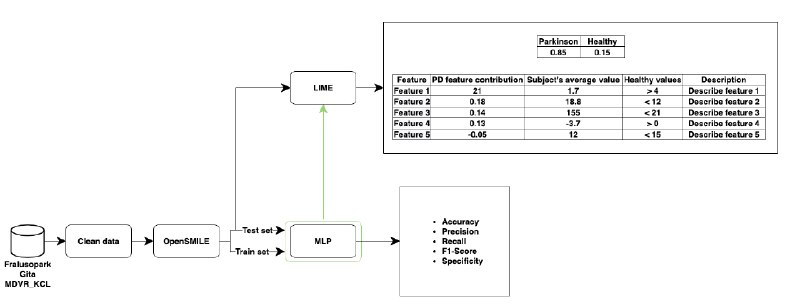
\includegraphics[clip=true, width=\textwidth]{figs/pipeline.png}
	\end{center}
	\caption{Pipeline of the proposed model.}
	\label{pipeline}
\end{figure*}

\pagebreak                       % adipisci velit

  %%%%%%%%%%%%%%%%%%%%%%%%%%%%%%%%%%%%%%%%%%%%%%%%%%%%%%%%%%%%%%%%%%%%%%%%%%%%%
  %
%%%%%                 P A R T E   I V  --  A V A L I A Ç Ã O
 %%%
  %

%
\part{Expedita Distinctio}
\thispagestyle{empty}
%\vbox to\textheight{
%\vfil
\chapter*{Omnis voluptas}
\thispagestyle{empty}

Et harum quidem rerum facilis est et expedita distinctio. Nam libero tempore, cum soluta nobis est eligendi optio, cumque nihil impedit, quo minus id, quod maxime placeat, facere possimus, omnis voluptas assumenda est, omnis dolor repellendus. Temporibus autem quibusdam et aut officiis debitis aut rerum necessitatibus saepe eveniet, ut et voluptates repudiandae sint et molestiae non recusandae. Itaque earum rerum hic tenetur a sapiente delectus, ut aut reiciendis voluptatibus maiores alias consequatur aut perferendis doloribus asperiores repellat.
%}
\newpage
\thispagestyle{empty}



%------------------------------------------------------------------------------
% Chapters are here
%
  %%%%%%%%%%%%%%%%%%%%%%%%%%%%%%%%%%%%%%% -*- coding: utf-8; mode: latex -*- %%
  %
%%%%%                       CHAPTER
 %%%
  %

\chapter{Results and discussion}
%\addcontentsline{lof}{chapter}{\thechapter\quad Nihil Molestiae}
%\addcontentsline{lot}{chapter}{\thechapter\quad Nihil Molestiae}
\label{ch:omnisvoluptas}

%\begin{quotation}
%  {\small\it Neque porro quisquam est qui dolorem ipsum quia dolor sit amet, consectetur, adipisci velit...}

%{\small\it -- Cerico}
%\end{quotation}


\section{Classification Experiments}

In this work, three types of experiments were conducted, each using two different architectures, as described in the previous chapter. Results are shown in tables \textbf{5.1} and \textbf{5.2} (for the baseline experiments), \textbf{5.3} and \textbf{5.4} (for the semi-independent experiments), and \textbf{5.5} and \textbf{5.6} (for the language-independent experiments). These tables show the five MLP parameter parameterizations with higher accuracy for each experiment. Tables \textbf{5.1}, \textbf{5.3} and \textbf{5.5} present the results for architecture 1, whereas tables \textbf{5.2}, \textbf{5.4} and \textbf{5.6} show the results for architecture 2.

\subsection{Baseline experiments}

Both architectures 1 and 2 of the \gls{mlp} yielded an accuracy of 90\% with the best parameterization (Tables \textbf{5.1} and \textbf{5.2}). \\
All the best models parameterizations (for both architectures 1 and 2) achieved higher scores using the GITA dataset. There are multiple reasons that can explain these results. In particular , the text read by subjects for the creation of the Gita dataset contains the complete set of Spanish sounds, which makes the data phonetically complete. Also, the audios from the MDVR\_KCL dataset were recorded using phone calls, which uses audio compression with data loss, resulting in a dataset with inferior quality. In addition, MDVR\_KCL has a significantly smaller recording time, which may limit the model learning. \\
The distribution between \gls{mlp} solvers (adam and lbfgs) on the top 5 model parameterizations for architecture 1 is similar, whereas 4 out of the 5 best model parameterizations on architecture 2 use the adam solver. Both architectures yielded better results when using valuer smaller values (0.0001 and 0.001) for the alpha parameter, comparing to the results obtained using larger values (0.1). Finally, architecture 1 does not show significant differences between models using 2000 and 5000 for the maximum number of iterations. In addition, this difference is observable on architecture 2, where the four model configurations which yielded better results by using the value of 5000 for this parameter regardless of the solver. The difference between architectures can be explained by the higher complexity of architecture 2 which require the optimization of a large number of parameters (52400 weights and 401 biases), compared with architecture 1, which has only 3844 weights and 63 bias. A larger number of parameters requires more iterations for the model's convergence. \\
Architecture 1 yielded precision values between 0.75 and 1, meaning that 75\% to 100\% of the patients labeled as \gls{pd} by the models were correctly classified. The precision of architecture 2 was slightly worse, between 67\% and 100\%. Recall values (which corresponds to the percentage of \gls{pd} patients were correctly classified) were similar for the two architectures. Architecture 1 led to recall values in the ranges [71-100]\% and [67-100]\%, respectively. Using the specificity metric (which corresponds to the percentage of \gls{hc} patients that were correctly classified) to compare the two architectures, architecture 2 outperformed architecture 1 by a small margin, producing a range of values between 80\% and 100\%, whereas architecture 1 produced a range of values between 75\% and 100\%. Finally, comparing both architectures using the F1-score metric, the performance of architecture 2 (up to 91\%) is usually higher than the one of architecture 2 (up to almost 86\%). \\
Overall, we can conclude that there are no significant differences between the two architectures.

\begin{table}
	\centering
	\begin{tabular}{lcccccccc}
		\bfseries dataset & \bfseries solver & \bfseries alpha & \bfseries max. iterations & \bfseries accuracy  & \bfseries precision & \bfseries recall & \bfseries specificity & \bfseries f1-score
		\csvreader[head to column names]{csvs/baseline_top.csv}{}
		{\\\hline\dataset & \solver & \alpha & \iterations & \accuracy  & \precision & \recall & \specificity & \fscore}
	\end{tabular}
	\caption{\label{tab:table-name}Baseline experiment results using architecture 1.}
\end{table}

\begin{table}
	\centering
	\begin{tabular}{lcccccccc}
		\bfseries dataset & \bfseries solver & \bfseries alpha & \bfseries max. iterations & \bfseries accuracy  & \bfseries precision & \bfseries recall & \bfseries specificity & \bfseries f1-score
		\csvreader[head to column names]{csvs/baseline_200_top.csv}{}
		{\\\hline\dataset & \solver & \alpha & \iterations & \accuracy  & \precision & \recall & \specificity & \fscore}
	\end{tabular}
	\caption{\label{tab:table-name}Baseline experiment result using architecture 2.}
\end{table}

\subsection{Semi-independent experiments}

When testing a semi-independent approach, architecture 1 yielded better results than architecture 2 (tables \textbf{table 5.3} and \textbf{table 5.4}). Although the two best model parameterization of both architectures produced an accuracy of 90\%, the following three model parameterization resulted in an accuracy of almost 86\%, whereas architecture 2 only reached an accuracy of 80\%. The same trend applies to precision.
\\
Architecture 1 outperformed architecture 2 on precision, producing results between 0.83 and 1, whereas architecture 2 yielded values between 0.6 and 1. While both architectures' highest value was the same, architecture 1 produced consistently better results, with a smaller range of values. Similar results were achieved when using recall. Architecture 1 produced values between 0.75 and 1, and 3 of the top 5 model parameterizations achieved 100\% recall. Additionally, architecture 2 values for recall ranged from 0.66 and 1. As F1-score combines the values from precision and recall (and architecture 1 outperformed architecture 2 on both these metrics), the F1-score metric leads to the same conclusions. Values of this metric for architecture 1 varied between 0.85 and 0.92, whereas architecture 2 values ranged from 0.75 to 0.88. Finally, architecture 2 produced better results when using specificity. This architecture's values varied between 0.71 and 1, with a much smaller variation between extremes when compared to the results produced by architecture 1, which varied from 0.5 to 1.
The results were similar to the ones achieved on the baseline experiences using architecture 2. Architecture 1 had a slightly better performance on the semi language-independent experiments, compared to the baselines.
This experiment confirms the conclusions of similar work that tested semi language-independent models \cite{parkinson_three_languages}, which suggests that these models can be retrained using a small dataset of a new language. These retrained models can be used on patients that speak the different language, without loss of performance. This characteristic can be particularly useful, as lack of training data is usually a limitation to train such models.

\begin{table}
	\centering
	\begin{tabular}{lcccccccc}
		\bfseries dataset & \bfseries solver & \bfseries alpha & \bfseries max. iterations & \bfseries accuracy  & \bfseries precision & \bfseries recall & \bfseries specificity & \bfseries f1-score
		\csvreader[head to column names]{csvs/semi_top.csv}{}
		{\\\hline\dataset & \solver & \alpha & \iterations & \accuracy  & \precision & \recall & \specificity & \fscore}
	\end{tabular}
	\caption{\label{tab:table-name}Semi-independent experiment result using architecture 1.}
\end{table}

\begin{table}
	\centering
	\begin{tabular}{lcccccccc}
		\bfseries dataset & \bfseries solver & \bfseries alpha & \bfseries max. iterations & \bfseries accuracy  & \bfseries precision & \bfseries recall & \bfseries specificity & \bfseries f1-score
		\csvreader[head to column names]{csvs/semi_200_top.csv}{}
		{\\\hline\dataset & \solver & \alpha & \iterations & \accuracy  & \precision & \recall & \specificity & \fscore}
	\end{tabular}
	\caption{\label{tab:table-name}Semi independent experiment result using architecture 2.}
\end{table}

\subsection{Language-independent experiments}

Language-independent models lead to substantially worse results compared to previous models (tables \textbf{table 5.5} and \textbf{table 5.6}). \\
When using a language-independent model, architecture 1 achieved a maximum accuracy of 67\%. Architecture 2 yielded very similar results, scoring a maximum of 66\% on this metric. \\
Combining the top five model parameterizations for both architectures, almost all (90\%) obtained their best scores when trained with the FraLusoPark and MDVR\_KCL, and tested with Gita. The same percentage of the combination of the top five models of each architecture used the \textit{lbfgs} solver, whereas only 1 of these 10 model parameterizations used the \textit{adam} solver. Similarly to the dependent and semi-independent experiments, the model's performance is consistently higher for smaller values of alpha. On both architectures, only 1 of the top five model parameterizations used $alpha = 1$. Finally, no significant differences were found when comparing model's performance based on the number of iterations. \\
Considering the precision metric, architecture 1 scored slightly higher values than architecture 2. It's values range between 0.59 and 0.64 whereas architecture 2 yielded values between 0.57 and 0.61, meaning that architecture 2 produced more false positives (patients from the \gls{hc} group incorrectly classified as \gls{pd}). Also, architecture 1 performed slightly worse when comparing the recall metric, only achieving values ranging from 0.76 to 0.84, whereas architecture 2 scored recall values between 0.77 and 0.88, thus correctly classifying a higher number of patients from the \gls{pd} group. Architecture 1 outperformed architecture 2, when compared using the specificity metric. Architecture 2 only achieved a maximum of 0.46, compared to architecture 1, which scored a maximum of 0.58 on this metric. Lastly, as F1-score combines precision and recall in the same metric, the results of both architectures on this metric were equivalent. \\
We can conclude that the models have a similar performance on the \gls{pd} detection task. Thus, Architecture 1 can be considered a better option for this task, as it is simpler, with only 3783 parameters to optimize, than architecture 2, which comprises a total of 52601 parameters. This difference makes architecture 1 much less resource-intensive, in both terms of time and computing power.

\begin{table}
	\centering
	\begin{tabular}{lcccccccc}
		\bfseries dataset & \bfseries solver & \bfseries alpha & \bfseries max. iterations & \bfseries accuracy  & \bfseries precision & \bfseries recall & \bfseries specificity & \bfseries f1-score
		\csvreader[head to column names]{csvs/independent_top.csv}{}
		{\\\hline\dataset & \solver & \alpha & \iterations & \accuracy  & \precision & \recall & \specificity & \fscore}
	\end{tabular}
	\caption{\label{tab:table-name}Independent experiment result using architecture 1.}
\end{table}

\begin{table}
	\centering
	\begin{tabular}{lcccccccc}
		\bfseries dataset & \bfseries solver & \bfseries alpha & \bfseries max. iterations & \bfseries accuracy  & \bfseries precision & \bfseries recall & \bfseries specificity & \bfseries f1-score
		\csvreader[head to column names]{csvs/independent_200_top.csv}{}
		{\\\hline\dataset & \solver & \alpha & \iterations & \accuracy  & \precision & \recall & \specificity & \fscore}
	\end{tabular}
	\caption{\label{tab:table-name}Independent experiment result using architecture 2.}
\end{table}

\subsection{Model optimization}

When comparing models' results per parameter, it is possible to find the best values for each parameter. \\
Smaller values for alpha (0.0001 and 0.001) consistently produced superior results when compared with 0.01. Considering language-dependent and semi language-dependent models, there is no clear difference between the use of the lbfgs and adam solvers. For both experiments, around half of the top five model parameterizations used each solver. In addition, for language-independent experiments, models using the lbfgs solver outperformed those using the adam solver. Between the top five model parameterizations of each architecture, only 1 was trained using adam (tables \textbf{5.5} and \textbf{5.6}). Lastly, comparing the results based on the number of maximum number of iterations ($\#interations$), there is no clear difference between models trained with $\#iterations = 2000$ and $\#iterations = 5000$ in any of the experiments performed. This shows that, in most cases, 2000 iterations should be sufficient to train the model, and convergence is reached without executing the maximum number of iterations.

\section{Language Independency}

Both architectures used during this work yielded an accuracy of 90\% on the semi language-independent experiments. One the one hand, these results are inferior to the ones achieved on a similar work (\cite{parkinson_three_languages}), where the authors were able to achieve a maximum accuracy of 96\% when training a model with a German dataset and 80\% of a Spanish dataset and testing with the remaining 20\%. On the other hand, this model was outperformed by architecture 1 when using the recall metric, producing recall values of 95\%, whereas architecture 1 produced a recall of 100\% for the top 3 model parameterizations. Contrary to this work, results produced by our model were inferior when using the specificity metric, where the authors were able to achieve a score of 97\%, compared to the 75\% produced by our model. Based on the recall metric, we can conclude that our solution has better ability to indicate when a subject belongs in the \gls{pd} group. This contrasts with the ability to classify subjects from the \gls{hc} group, where our model has an inferior performance. As previously described in section 5.1.3, architecture 1 produced an accuracy of 67\% on the language-independent experiments. This result is slightly inferior to the one achieved on a different article \cite{parkinson_three_languages}, where a language-independent model yielded an accuracy of 77\% when trained with a Czech dataset and tested with a German dataset. Comparing the models using the recall and specificity metrics, the results are identical to the ones achieved on the semi language-independent models' comparison in this work. Our model produced a recall of 76\% whereas the authors were only able to score 53\% on this metric. On the other hand, architecture 1 produced a score of 58\% on the specificity metric, significantly inferior to the 95\% achieved by the other work. \\
It is possible to conclude that the performance of both architectures used in this work were not able to produce results at the state-of-the-art on the language independency topic. Regarding the recall metric, both architectures outperformed the state-of-the-art, which demonstrates better capacity in detecting \gls{pd}.

\section{Explainability}

LIME was used to generate explanations for each test subject. These are local explanations, as they are able to explain the classification of each test subject. Results obtained following this process are described in section 5.3.1. By analyzing the complete set of explanations produced in this work, the global contribution (weight) of each feature was evaluated for the classification. Results for the global analysis are described in section 5.3.2.

\subsection{Local Explanations}

\begin{figure*}[t]
	\begin{center}
		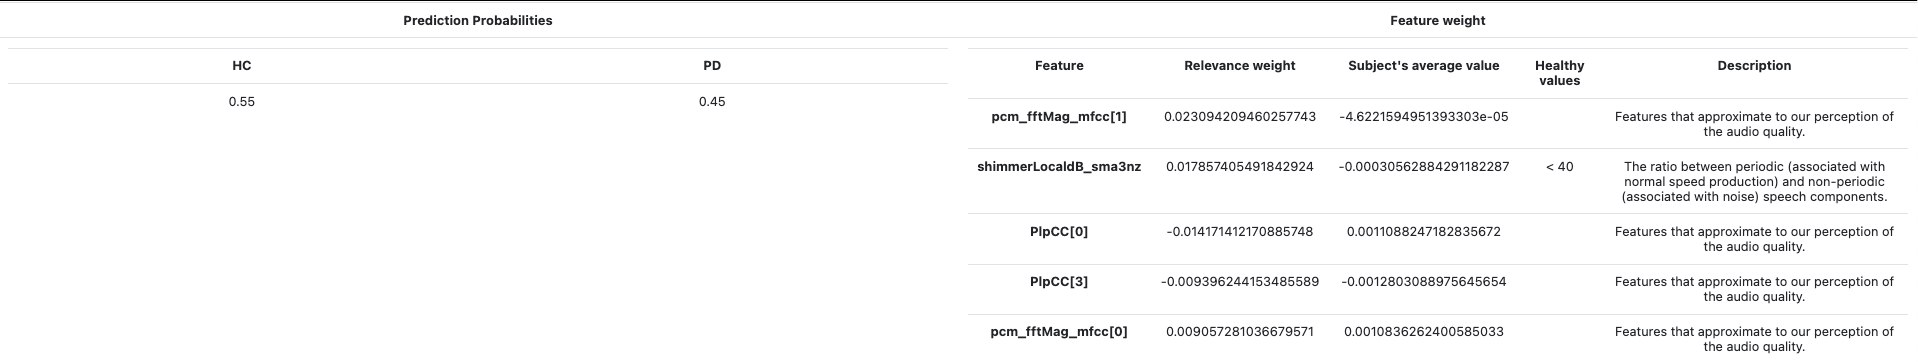
\includegraphics[clip=true, width=\textwidth]{figs/example_explanation.png}
	\end{center}
	\caption{Example of an explanation generated by LIME.}
	\label{explanation}
\end{figure*}

To generate an explanation, the top 5 features with the highest contribution to the diagnostic are selected. Figure \ref{explanation} illustrates an explanation, containing the percentage attributed to each class (\gls{pd} and \gls{hc}), the features with the highest contribution to the diagnostic, their corresponding weights, the subject's average value on that feature, the range of normal values for a healthy subject (extracted from the bibliography), and a short description of the feature. This information provides a clearer insight of the model's
classification to the medical professional. The percentage attributed to each class allows to evaluate the degree of confidence of the model in the decision, whereas the average features values can be compared to the normal range of values to check for abnormal parameters. Finally, the feature description links the mathematical definition of the features with its physical manifestation, thus simplifying the interpretation of the results by the medical professional. 

\subsection{Global Feature Contribution}

\begin{table}
	\centering
	\begin{tabular}{lcccccccc}
		\bfseries feature & \bfseries percentage of subjects & \bfseries contribution (weight)
		\csvreader[head to column names]{csvs/explanation_by_percentage.csv}{}
		{\\\hline\feature & \percentage & \weight}
	\end{tabular}
	\caption{\label{tab:table-name}Top 10 more common features on explanations.}
\end{table}

\begin{table}
	\centering
	\begin{tabular}{lcccccccc}
		\bfseries feature & \bfseries percentage of subjects & \bfseries contribution (weight)
		\csvreader[head to column names]{csvs/explanation_by_weight.csv}{}
		{\\\hline\feature & \percentage & \weight}
	\end{tabular}
	\caption{\label{tab:table-name}Top 10 features ordered by contribution (weight) to explanations.}
	
\end{table}

The top 10 features were sorted by their frequency on the complete set of explanations produced in this work and by average contribution to the models' classification, (Tables 5.7 and 5.8). \\
\gls{plp} and \gls{mfcc} are different mathematical representations of sound that simulate the way humans perceive it. These two sets of features constitute the majority of the top features with highest contribution to the largest number of test subjects (tables 5.7 and 5.8).
Comparing the \gls{mfcc}s (represented on the table as \textit{pcm\_fftMag\_mfcc[n]}) and \gls{plp}s (represented on the table as \textit{PlpCC[n]}), there are no significant differences between these features. In addition, jitter (\textit{jitterLocal\_sma3nz}) is also on the top features with higher weight contribution. Finally, \gls{f0}, shimmer and \gls{hnr} produce significant contributions to few test subjects (8.2\% for F0, 7.4\% for shimmer and 6.5\% for HNR). These features' contributions are inferior to the ones shown on the table (0.0437 for F0, 0.0402 for HNR and 0.0379 for shimmer). \\
The global contribution (weight) for each feature can be observed in figure \ref{weight}. The weight of the feature with highest global contribution is around 66\% larger than the weight from the feature with lowest contribution. In addition, there is a significant difference between the weight of the top three features and the others, which can be defined as a threshold to separate the features into two groups (\textit{relevant} and \textit{irrelevant}). \\
The small difference between contribution (weight) values for consecutive features suggests a correlation between some features. The same trend applies when sorting features by percentage of subjects. \\ 
The best performing features are similar in both analysis, with a strong presence of MFCC and PLP group of features. A significant difference can be observed between the 5\textsuperscript{th} and the 6\textsuperscript{th} top features, which can also be defined as the threshold to separate the features into \textit{relevant} and \textit{irrelevant} groups. \\
Combining both analysis, the combined threshold can be defined as the top 5 features, meaning that this should be the group of features that the medical professional should focus on.

\begin{landscape}
	\begin{figure*}[t]
		\begin{center}
			%\scalebox{1}[-1]{ 
				%\scalebox{-1}[1]{
				    \rotatebox[origin=c]{180}{
						\includegraphics[clip=false,height=0.95\textwidth,width=0.95\textwidth]{figs/feature_by_weight.png}
					}
				%}
			%}
		\end{center}
		\caption{Global contribution (weight) by feature.}
		\label{weight}
	\end{figure*}
\end{landscape}

\begin{landscape}
	\begin{figure*}[t]
		\begin{center}
			%\scalebox{1}[-1]{ 
			%\scalebox{-1}[1]{
			\rotatebox[origin=c]{180}{
				\includegraphics[clip=false,height=0.95\textwidth,width=0.95\textwidth]{figs/feature_by_percentage.png}
			}
			%}
			%}
		\end{center}
		\caption{Percentage of subjects by feature.}
		\label{percentage}
	\end{figure*}
\end{landscape}

                   % omnis voluptas
  %%%%%%%%%%%%%%%%%%%%%%%%%%%%%%%%%%%%%%% -*- coding: utf-8; mode: latex -*- %%
  %
%%%%%                       CHAPTER
 %%%
  %

\chapter{Conclusions}
%\addcontentsline{lof}{chapter}{\thechapter\quad Nihil Molestiae}
%\addcontentsline{lot}{chapter}{\thechapter\quad Nihil Molestiae}
\label{ch:magna}

%\begin{quotation}
%  {\small\it Neque porro quisquam est qui dolorem ipsum quia dolor sit amet, consectetur, adipisci velit...}

%{\small\it -- Cerico}
%\end{quotation}

Future work:
 - Add meta features, such as gender, that condition the normal value of a feature (such as F0)
 - Extend this work to generate global explanations at the same time
 - Test simpler features, such as log-filter bank (instead of MFCC) and compare accuracies. These would be easier to explain

  %
 %%%
%%%%%                           THE END
  %
  %%%%%%%%%%%%%%%%%%%%%%%%%%%%%%%%%%%%%%%%%%%%%%%%%%%%%%%%%%%%%%%%%%%%%%%%%%%%%

%%% Local Variables: 
%%% mode: latex
%%% TeX-master: "tese"
%%% End: 
                               % magna aliqua

  %%%%%%%%%%%%%%%%%%%%%%%%%%%%%%%%%%%%%%%%%%%%%%%%%%%%%%%%%%%%%%%%%%%%%%%%%%%%%
  %
%%%%%                    BIBLIOGRAPHY AND AUTHOR INDEX
 %%%
  %
  
%---------------------------------------------------------------------------
% Bibliography styles
%
%\bibliographystyle{authordate}
%\bibliographystyle{chicago}
\bibliographystyle{apacitex}


%---------------------------------------------------------------------------
% Bibliographics databases
%
\bibliography{refs/document}

%---------------------------------------------------------------------------
\begin{singlespace}
\printindex[autx]\cleardoublepage            % Author index (apacite)
\end{singlespace}

  %%%%%%%%%%%%%%%%%%%%%%%%%%%%%%%%%%%%%%%%%%%%%%%%%%%%%%%%%%%%%%%%%%%%%%%%%%%%%
  %
%%%%%                         APPENDIX
 %%%
  %

\part{Appendices}
\appendix

%  %%%%%%%%%%%%%%%%%%%%%%%%%%%%%%%%%%%%%%% -*- coding: utf-8; mode: latex -*- %%
  %
%%%%%                     APPENDIX
 %%%
  %

\chapter{Commodo Consequat}
%\addcontentsline{lof}{chapter}{\thechapter\quad Commodo Consequat}
%\addcontentsline{lot}{chapter}{\thechapter\quad Commodo Consequat}
\label{ch:commodo}

\begin{figure}[htb]
  \centering
  %\includegraphics[width=\textwidth]{finame.eps}
  \caption{Soluta nobis est eligendi optio.}
  \label{fig:soluta-nobis}
\end{figure}

         % commodo consequat

%\begin{singlespace}
%\printnomenclature\cleardoublepage               % Glossary
%\end{singlespace}

\begin{singlespace}
\printglossary[type=\acronymtype,title={\protect\centering\glossaryname}]\cleardoublepage
\end{singlespace}


\begin{table}[!htb]
	\renewcommand{\arraystretch}{1.3} % more space between rows
	\centering
	\begin{tabular}{lcc}
		\hline
		~       & Male & Female \\ \hline
		F0 (Hz)      & 105-160 & 175-245 \\ 
		Jitter (\%)  & \multicolumn{2}{c}{ $<$ 1.04  } \\ 
		Shimmer (\%) & \multicolumn{2}{c}{ $<$ 3.81 } \\
		HNR (dB)     & \multicolumn{2}{c}{ $<$ 20 (/a/, /i/), $<$ 40 (/u/) } \\
		\hline
	\end{tabular}
	\caption[Feature values for healthy subjects.]{Feature values for healthy subjects.}
	\label{normalValues}
\end{table}

\pagebreak

\begin{table}[!htb]
	\renewcommand{\arraystretch}{1.4} % more space between rows
	\centering
	\begin{tabular}{cL}
		\hline
		~ & \textbf{Description} \\ \hline
		F0      & The number of open/close cycles of the glottis. \\ 
		Jitter  & Measures the frequency variation between cycles. Affected by lack of control on the vocal cords vibration. \\ 
		Shimmer & Measures the amplitude variation between cycles. \\ 
		HNR     & The ratio between periodic (associated with normal speed production) and non-periodic (associated with noise) speech components. \\ 
		MFCC    & Features that approximate to our perception of the audio quality \\ 
		PLP     & Features that approximate to our perception of the audio quality \\
		\hline
	\end{tabular}
	\caption[Acoustic features description.]{Acoustic features description.}
	\label{featureDescription}
\end{table}

  %%%%%%%%%%%%%%%%%%%%%%%%%%%%%%%%%%%%%%%%%%%%%%%%%%%%%%%%%%%%%%%%%%%%%%%%%%%%%
  %
%%%%%                         SPECIAL
 %%%
  %
\begin{singlespace}

\def\indexname{Index}             % Index
\printindex\cleardoublepage

\end{singlespace}

\end{document}

  %
 %%%
%%%%%                          THE END
  %
  %%%%%%%%%%%%%%%%%%%%%%%%%%%%%%%%%%%%%%%%%%%%%%%%%%%%%%%%%%%%%%%%%%%%%%%%%%%%%
